\PassOptionsToPackage{dvipsnames}{xcolor}
\documentclass[notes]{beamer}
\usepackage{tikz}
\usetheme{_SalmanWarsaw}
\setbeamertemplate{navigation symbols}{}
%\setbeamertemplate{background}[grid][step=1cm] %default  page size in Beamer is 128mm x 96mm, with an 8 mm grid, this is 16x12

\usepackage[absolute,overlay]{textpos}
\usepackage{graphicx, url}
\usepackage[backend=bibtex]{biblatex}
\defbibheading{bibliography}[\bibname]{} %this prevents \printbibliography from producing an extra section
\bibliography{MyCitations}
\usepackage{animate}
\usepackage{appendixnumberbeamer}


\definecolor{darkgreen}{rgb}{0,0.5,0}

%page numbers
\newcommand{\mypagenumwhite}
{
\begin{textblock*}{1in}(4.4in, 0.02in)
{\small \color[rgb]{1,1,1}{\insertframenumber~/~\inserttotalframenumber}} 
\end{textblock*}
}
\newcommand{\mypagenumblack}
{
\begin{textblock*}{1in}(4.4in, 0.02in)
{\small \color[rgb]{0,0,0}{\insertframenumber~/~\inserttotalframenumber}} 
\end{textblock*}
}
   
%write ``extra slides'' on extra slides   
\newcommand{\extraslides}
{
\begin{textblock*}{1in}(0.1in, 0.02in)
{\large \color[rgb]{1,0,0}{Extra slides}}
\end{textblock*}
}
 
%change margin 
\newenvironment{changemargin}[2]
{
  	\begin{list}{}
{
\setlength{\topsep}{0pt}%
\setlength{\leftmargin}{#1}%
\setlength{\rightmargin}{#2}%
\setlength{\listparindent}{\parindent}%
\setlength{\itemindent}{\parindent}%
\setlength{\parsep}{\parskip}%
}
  	\item[]
}
{\end{list}
}    
    
%how to cite    
\newcommand{\myciteurl}[1]
{
	\tiny \citeauthor{#1}, \citetitle{#1}, \citeurl{#1}
}

\setbeamertemplate{itemize/enumerate body begin}{\setlength{\leftmargini}{-0.1cm}}
\setbeamercolor{block title}{bg=blue}
%\setbeamercolor{block title}{bg=Bittersweet}
\definecolor{darkgreen}{rgb}{0,0.5,0}

\newcommand{\Ainvertedhat}{\stackrel{\mathrel{\raisebox{.001in}{\reflectbox{\rotatebox[origin=c]{180}{$\hat{}$}}}}}{A}}

\newcommand{\muone}{{\color{red}\mu_1}}
\newcommand{\mutwo}{{\color{blue}\mu_2}}
\newcommand{\mufused}{{\color{darkgreen}\mu_{fused}}}



\newcommand{\sone}{{\color{red}\sigma_1}}
\newcommand{\stwo}{\color{blue}{\sigma_2}}
\newcommand{\sfused}{{\color{darkgreen}\sigma_{fused}}}


\newcommand{\varone}{{\color{red}\sigma^2_1}}
\newcommand{\vartwo}{{\color{blue}\sigma^2_2}}
\newcommand{\varfused}{{\color{darkgreen}\sigma_{fused}^2}}


\newcommand{\varsum}{{\color{darkgreen}{\varone + \vartwo}}}
\newcommand{\varprod}{{\color{darkgreen}{\varone \vartwo}}}

\newcommand{\divvarprodvarsum}{\color{darkgreen}    2\frac {\varprod}{\varsum} 	}

\newcommand{\xx}{\color{darkgreen}{\frac{ - \frac { \sigma_2^2 }{\sigma_1^2 + \sigma_2^2} (x-\mu_1)^2 - \frac{ \sigma_1^2 }{\varsum} (x-\mu_2)^2 } \divvarprodvarsum }}

\newcommand{\myalpha}{{\color{red}\ln ( 2 \pi ( \varone + \vartwo ) )}}



\newcommand{\CTFS}{\frac{1}{T}\bigints\limits_T {\color{blue}x(t)}e^{-jk\omega_0 t}dt}
\newcommand{\DTFS}{\frac{1}{N}\sum\limits_N  {\color{blue}x\left[n\right]} e^{-jk\omega_0 n}}
\newcommand{\CTFT}{\bigints\limits_{\textrm{-}\infty}^{\infty} {\color{blue}x(t)}e^{-j\omega t}dt}
\newcommand{\DTFT}{\sum\limits^{\infty}_{n=\textrm{-}\infty} {\color{blue}x\left[n\right]}e^{-j\omega n}}

\newcommand{\ICTFS}{\sum\limits_{k=\textrm{-}\infty}^{\infty}{\color{lightblue}X[k]}e^{jk\omega_0 t}}
\newcommand{\IDTFS}{\sum\limits_N  {\color{lightblue}X[k]} e^{jk\omega_0 n}}
\newcommand{\ICTFT}{\frac{1}{2\pi}\bigints\limits_{\textrm{-}\infty}^{\infty} {\color{lightblue}X(j\omega)}e^{j\omega t}d\omega}
\newcommand{\IDTFT}{\frac{1}{2\pi}\bigints_{2\pi} {\color{lightblue}X(e^{j\omega})} e^{j\omega n}d\omega}

\newcommand{\sT}{\bigints\limits_{\textrm{-}\infty}^{\infty} {\color{blue}x(t)}e^{-st}dt}
\newcommand{\IsT}{\frac{1}{2\pi j} \bigints\limits_{\sigma\textrm{-}j\omega}^{\sigma+j\omega} X(s)e^{st}ds}
\newcommand{\zT}{\sum\limits^{\infty}_{n=\textrm{-}\infty} {\color{blue}x\left[n\right]}z^{-n}}

\newcommand{\argmin}{\operatornamewithlimits{argmin}}

\newcommand{\A}{\textbf{A}}
\newcommand{\B}{\textbf{B}}
\newcommand{\C}{\textbf{C}}
\newcommand{\D}{\textbf{D}}
\newcommand{\F}{\textbf{F}}
\newcommand{\X}{\textbf{X}}
\newcommand{\Y}{\textbf{Y}}
\newcommand{\I}{\textbf{I}}
\newcommand{\bL}{\textbf{L}}
\newcommand{\U}{\textbf{U}}
\newcommand{\bu}{\textbf{u}}
\newcommand{\G}{\textbf{G}}
\newcommand{\M}{\textbf{M}}
\newcommand{\N}{\textbf{N}}
\newcommand{\x}{\textbf{x}}
\newcommand{\p}{\textbf{p}}
\newcommand{\rx}{{\color{red}\textbf{x}}}
\newcommand{\e}{\textbf{e}}
\newcommand{\xh}{\hat{\textbf{x}}}
\newcommand{\K}{\textbf{K}}
\newcommand{\bP}{\textbf{P}}
\newcommand{\bH}{\textbf{H}}
\newcommand{\R}{\textbf{R}}
\newcommand{\Q}{\textbf{Q}}
\newcommand{\CsIAB}{\C{\color{darkgreen}(s\I-\A)^{-1}}\B}
\newcommand{\sIA}{{\color{darkgreen}(s\I-\A)}}
\newcommand{\ut}{\tilde{u}}
\newcommand{\w}{\textbf{w}}
\newcommand{\yt}{\tilde{y}}
\newcommand{\zmone}{z^{-1}} 
\newcommand{\zmtwo}{z^{-2}} 
\newcommand{\bzm}{{\color{blue}z^{-1}}} 
\newcommand{\rzm}{{\color{red}z^{-1}}} 
\newcommand{\emT}{e^{-T}} 
\newcommand{\ABCD}{\center
$\boxed{\begin{array}{rll}
\dot{\textbf{x}}&=& \textbf{Ax+B}u\\
{\textbf{y}}&=& \textbf{Cx+D}u
\end{array}}
$}
\newcommand{\esT}{{\color{red}e^{sT}}} 
\newcommand{\emsT}{{\color{red}e^{-sT}}} 

\newcommand{\mybaa}{{\color{Purple}(\x-\xh)}}
\newcommand{\myaa}{{\color{Purple}(x-\hat{x})}}

\newcommand{\mPhi}{{\color{brown}\phi}} %m for motor
\newcommand{\mOmega}{{\color{blue}\omega}}
\newcommand{\mA}{{\color{blue}A}}
\newcommand{\mB}{{\color{brown}B}}
\newcommand{\mEA}{{\color{red}E_A}}
\newcommand{\mVA}{{\color{red}V_A}}
\newcommand{\mVF}{{\color{red}V_F}}
\newcommand{\mVT}{{\color{red}V_T}}
\newcommand{\mVB}{{\color{red}V_B}}
\newcommand{\mIF}{{\color{darkgreen}I_F}}
\newcommand{\mIA}{{\color{darkgreen}I_A}}
\newcommand{\mIL}{{\color{darkgreen}I_L}}
\newcommand{\mK}{{\color{blue}K}}
\newcommand{\mTauInd}{{\color{blue}\tau_{ind}}}
\newcommand{\mTauLoad}{{\color{blue}\tau_{load}}}
\newcommand{\mTauNet}{{\color{blue}\tau_{net}}}

\newcommand{\mTorque}{\mTauInd=\mK\mPhi\mIA}
\newcommand{\mIAmot}{\mIA=\frac{\mVB-\mEA}{R_A}}
\newcommand{\mIAgen}{\mIA=\frac{\mEA-\mVB}{R_A}}
\newcommand{\mInducedVoltage}{\mEA=\mK\mPhi\mOmega}
\newcommand{\mEAratioOne}{\frac{{\mEA}_1}{{\mEA}_2} = \frac{\mK\mPhi_1\mOmega_1}{\mK\mPhi_2\mOmega_2}}
\newcommand{\mEAratioTwo}{\frac{{\mEA}_1}{{\mEA}_2} &=& \frac{\mK\mPhi_1\mOmega_1}{\mK\mPhi_2\mOmega_2}}

\newcommand{\mLorentz}{{\color{blue}\mathbf{F}} = \mIA({\color{blue}\boldsymbol{\ell}} \times \mB)}



\title{Data Fusion\\
An Intuitive Look}  
\author{Dr Salman Aslam}
\date{} 



%##################################
\begin{document}
%##################################
\begin{frame}[plain]\pw\Large
\vspace{0.8in}
\titlepage
\end{frame}

\begin{frame}[plain]\pw\Large
\frametitle{\textbf{Sequence}}
\setcounter{tocdepth}{1}
\tableofcontents
\end{frame} 

\begin{frame}[plain]\pw\Large
\frametitle{\textbf{Sequence : detailed}}
\setcounter{tocdepth}{2}
\tableofcontents%[pausesections]
\end{frame} 

%###############
\section{Introduction}
%###############

%=================
\subsection{Notation}
%=================
\begin{frame}\pw\Large
\frametitle{Overview}
\framesubtitle{}
\begin{figure}
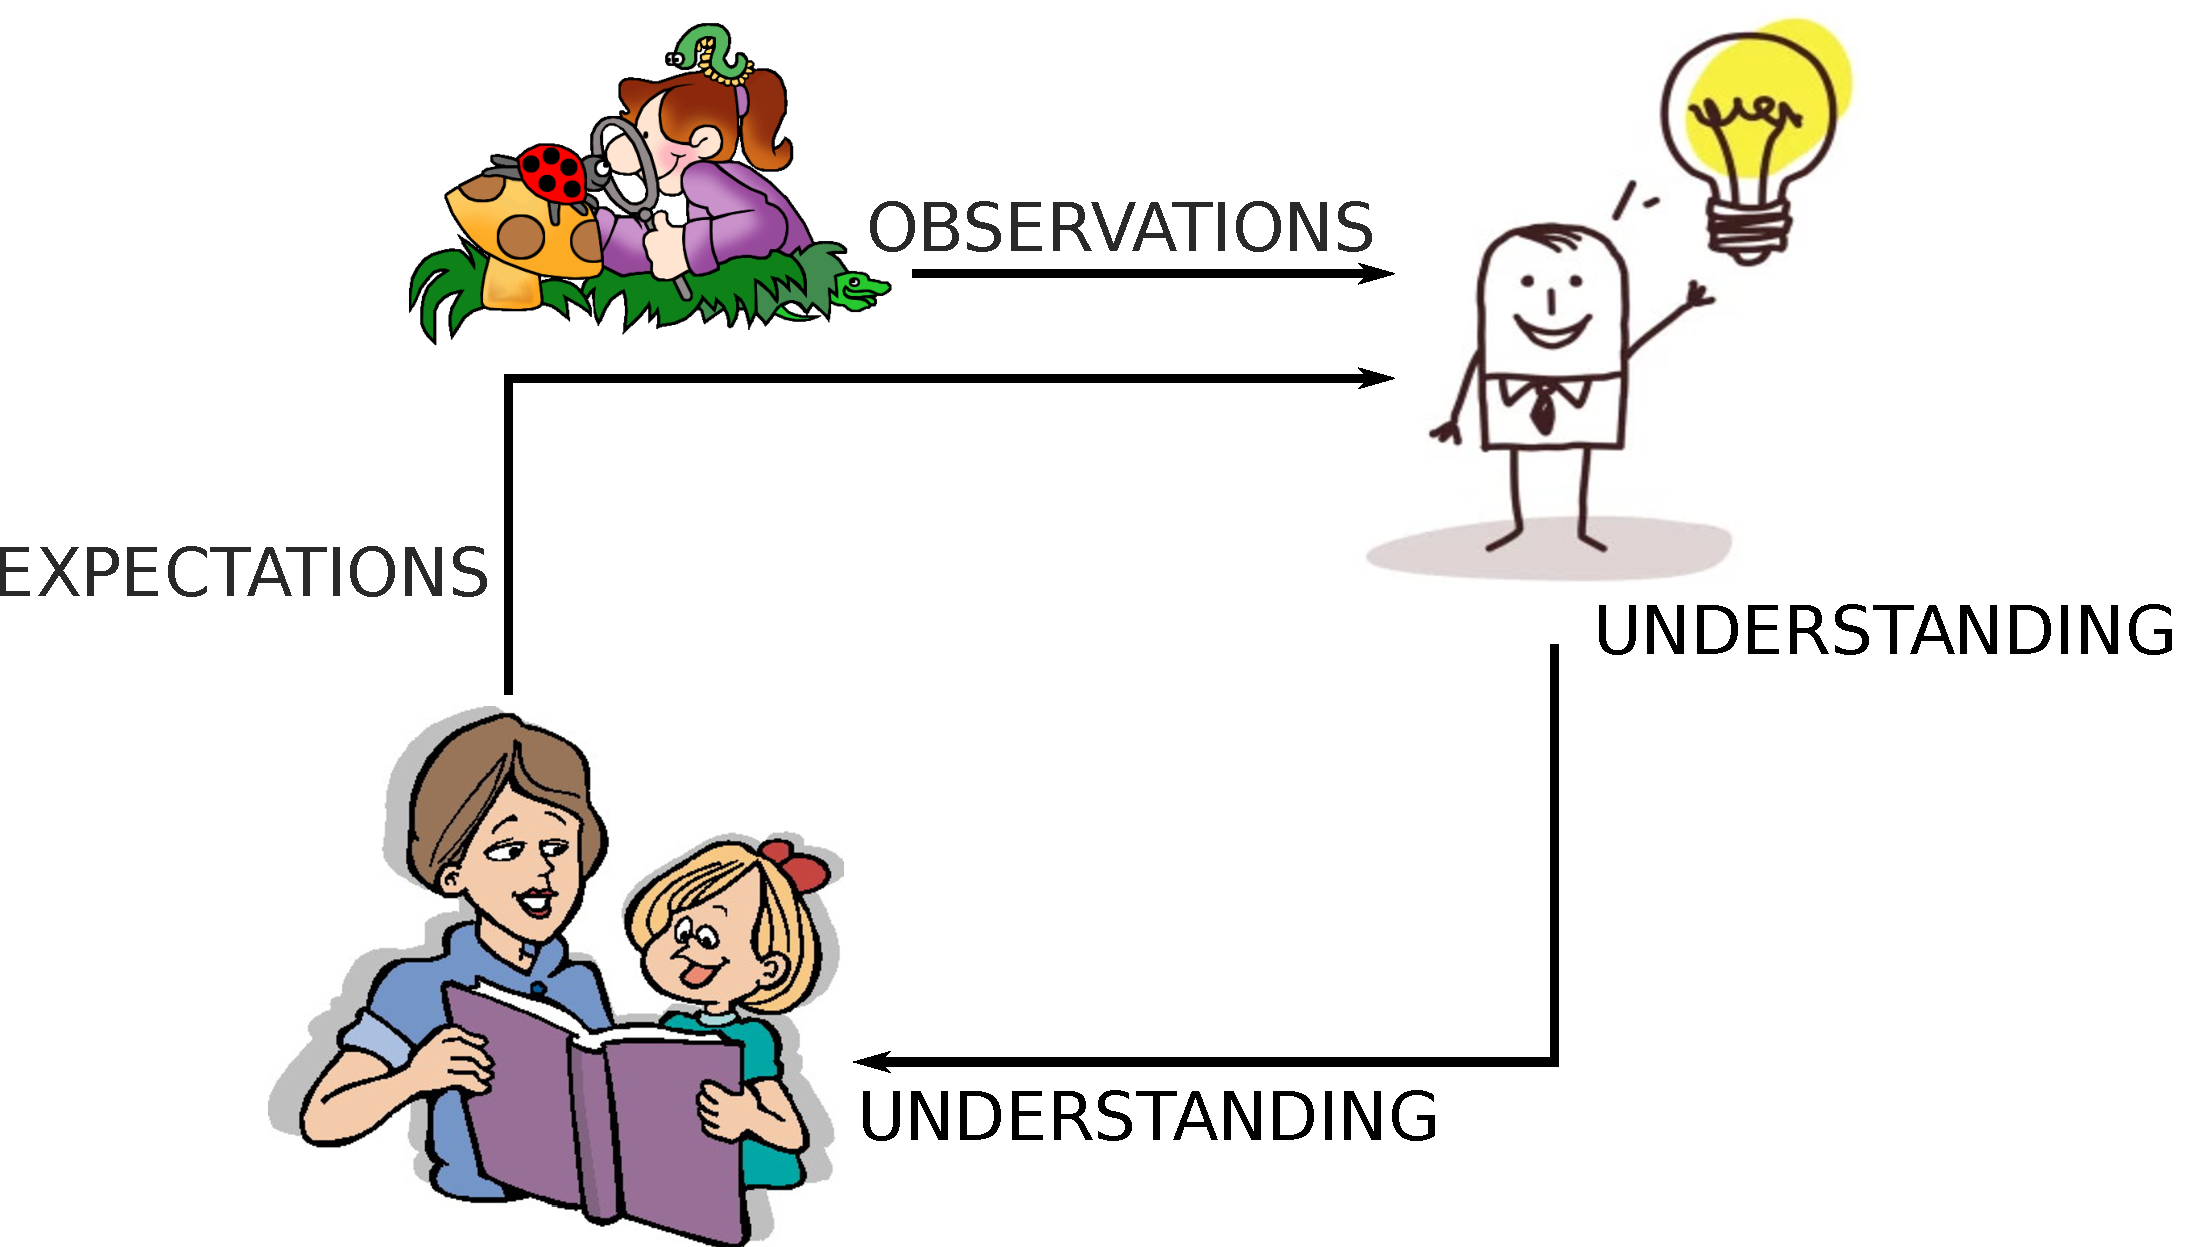
\includegraphics[width=0.95\textwidth]{figs/WFAR11_UCP_Update_Prediction_1_Notation-1.pdf}
\end{figure}
\end{frame}


\begin{frame}\pw\Large
\frametitle{Overview}
\framesubtitle{}
\begin{figure}
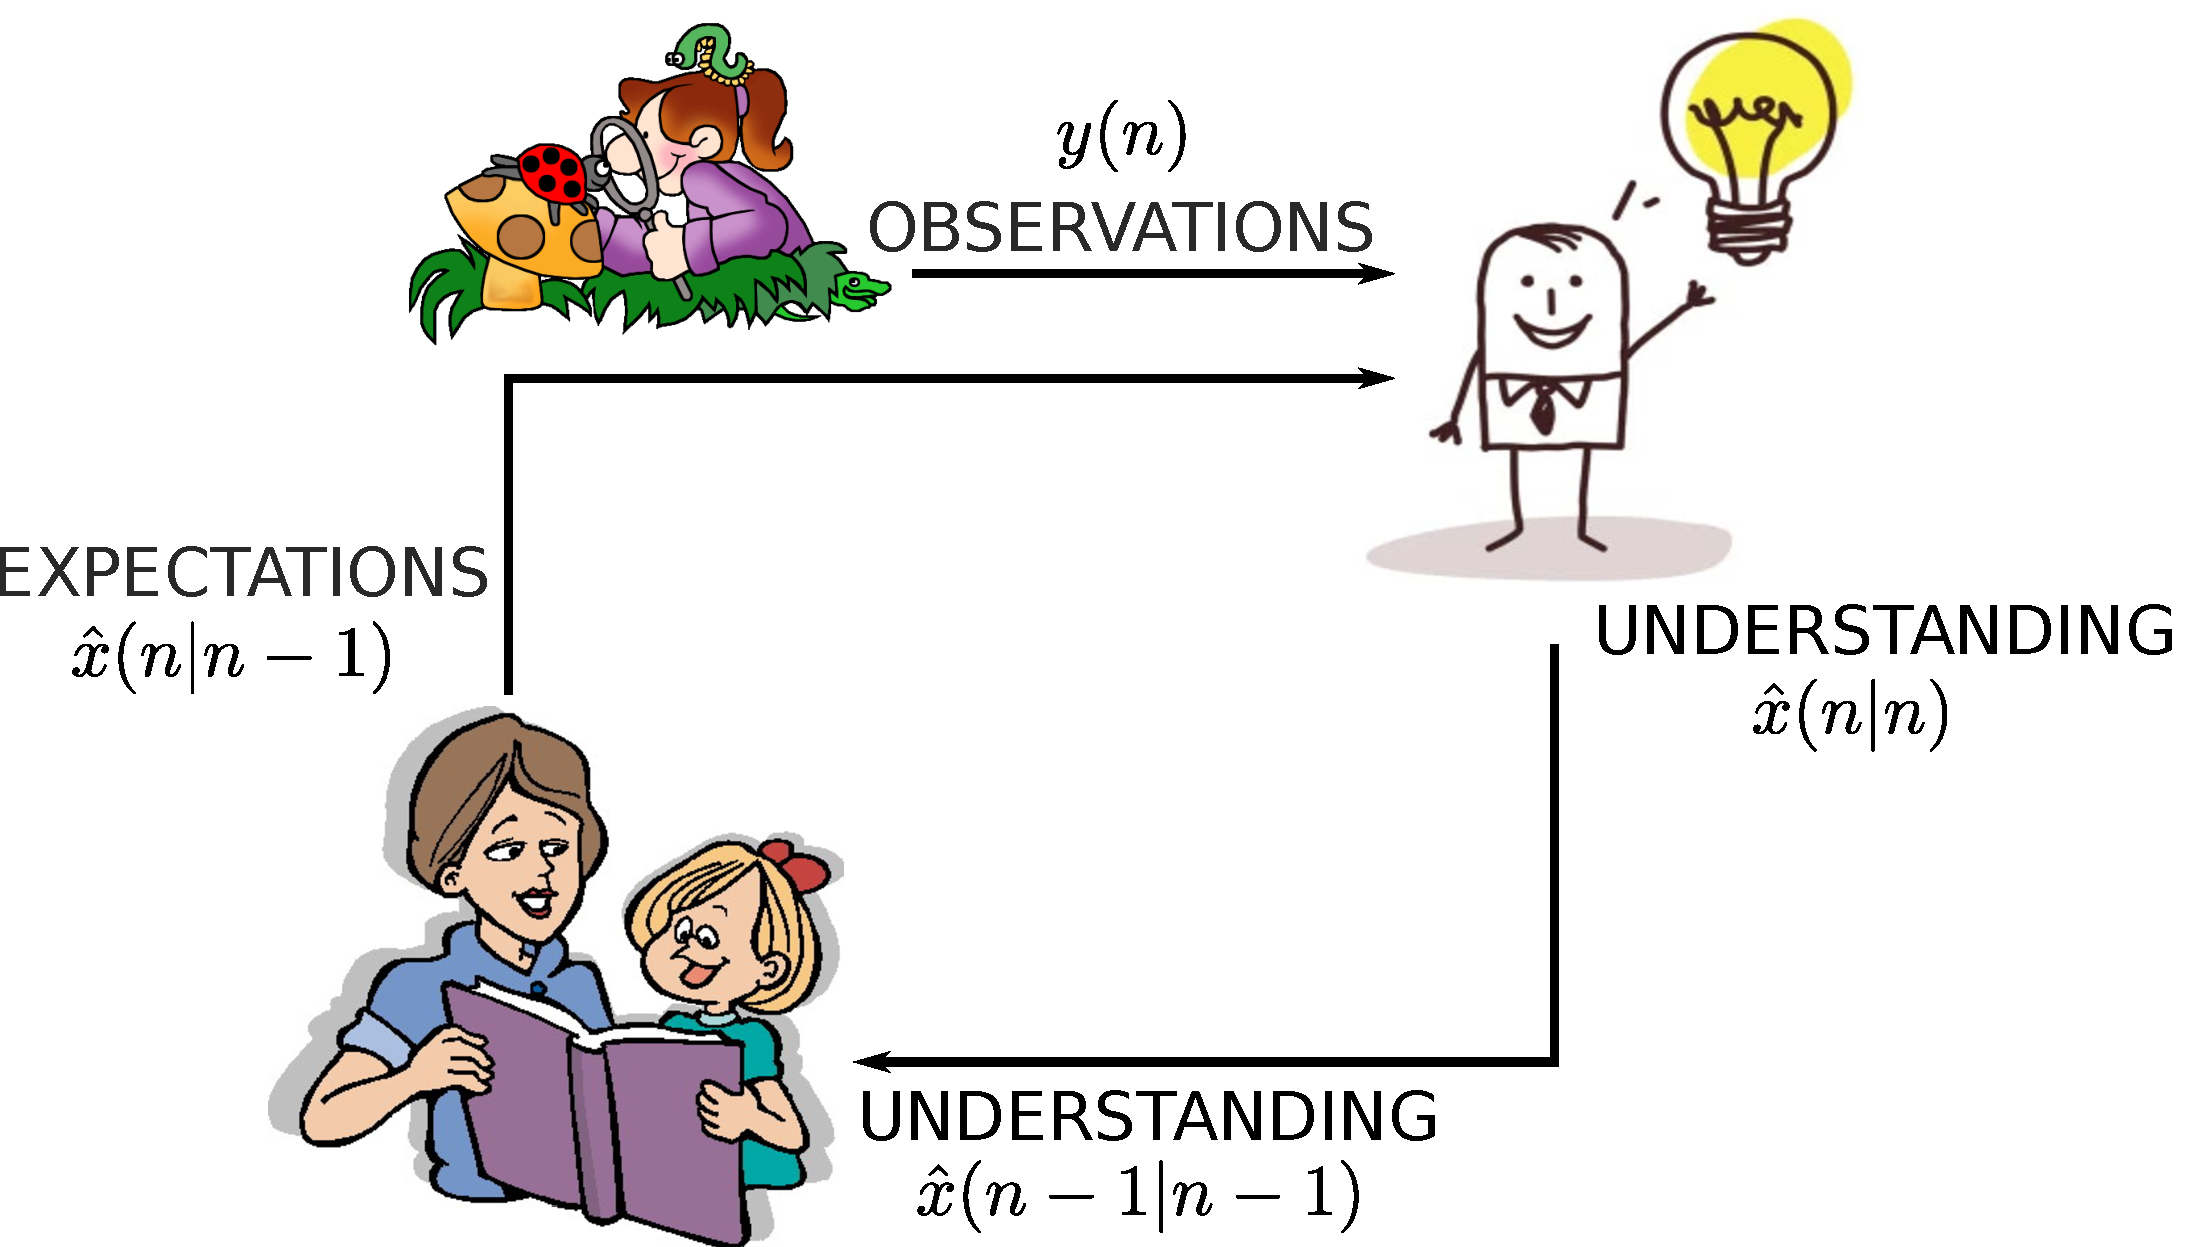
\includegraphics[width=0.95\textwidth]{figs/WFAR11_UCP_Update_Prediction_1_Notation-2.pdf}
\end{figure}
\end{frame}



\begin{frame}\pw\Large
\frametitle{Overview}
\framesubtitle{}
\begin{figure}
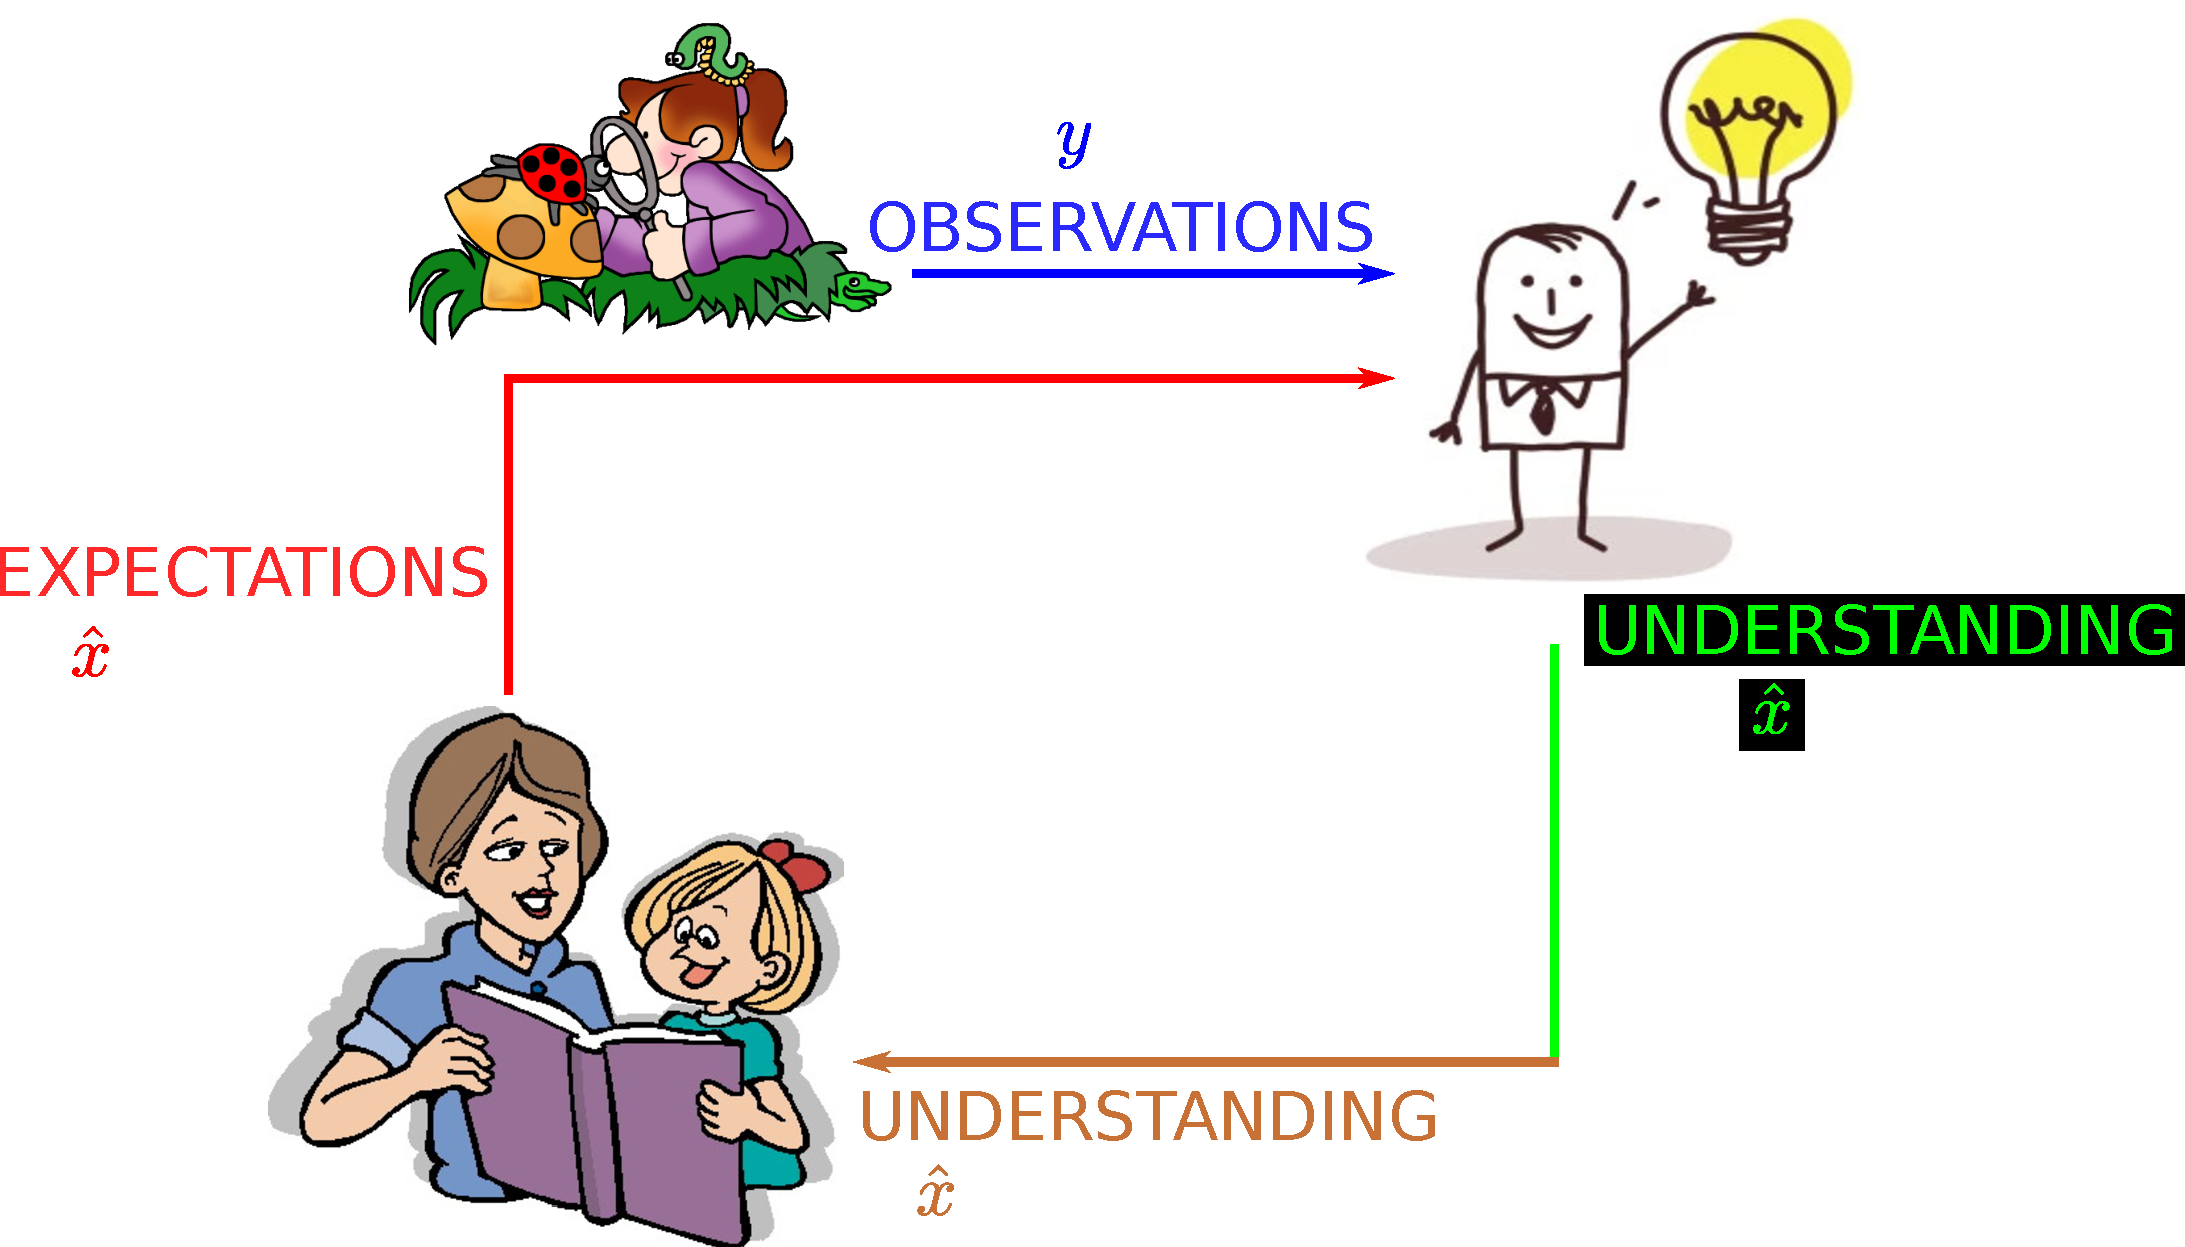
\includegraphics[width=0.95\textwidth]{figs/WFAR11_UCP_Update_Prediction_1_Notation-3.pdf}
\end{figure}
\end{frame}



\begin{frame}\pw\Large
\frametitle{Overview}
\framesubtitle{}
\begin{figure}
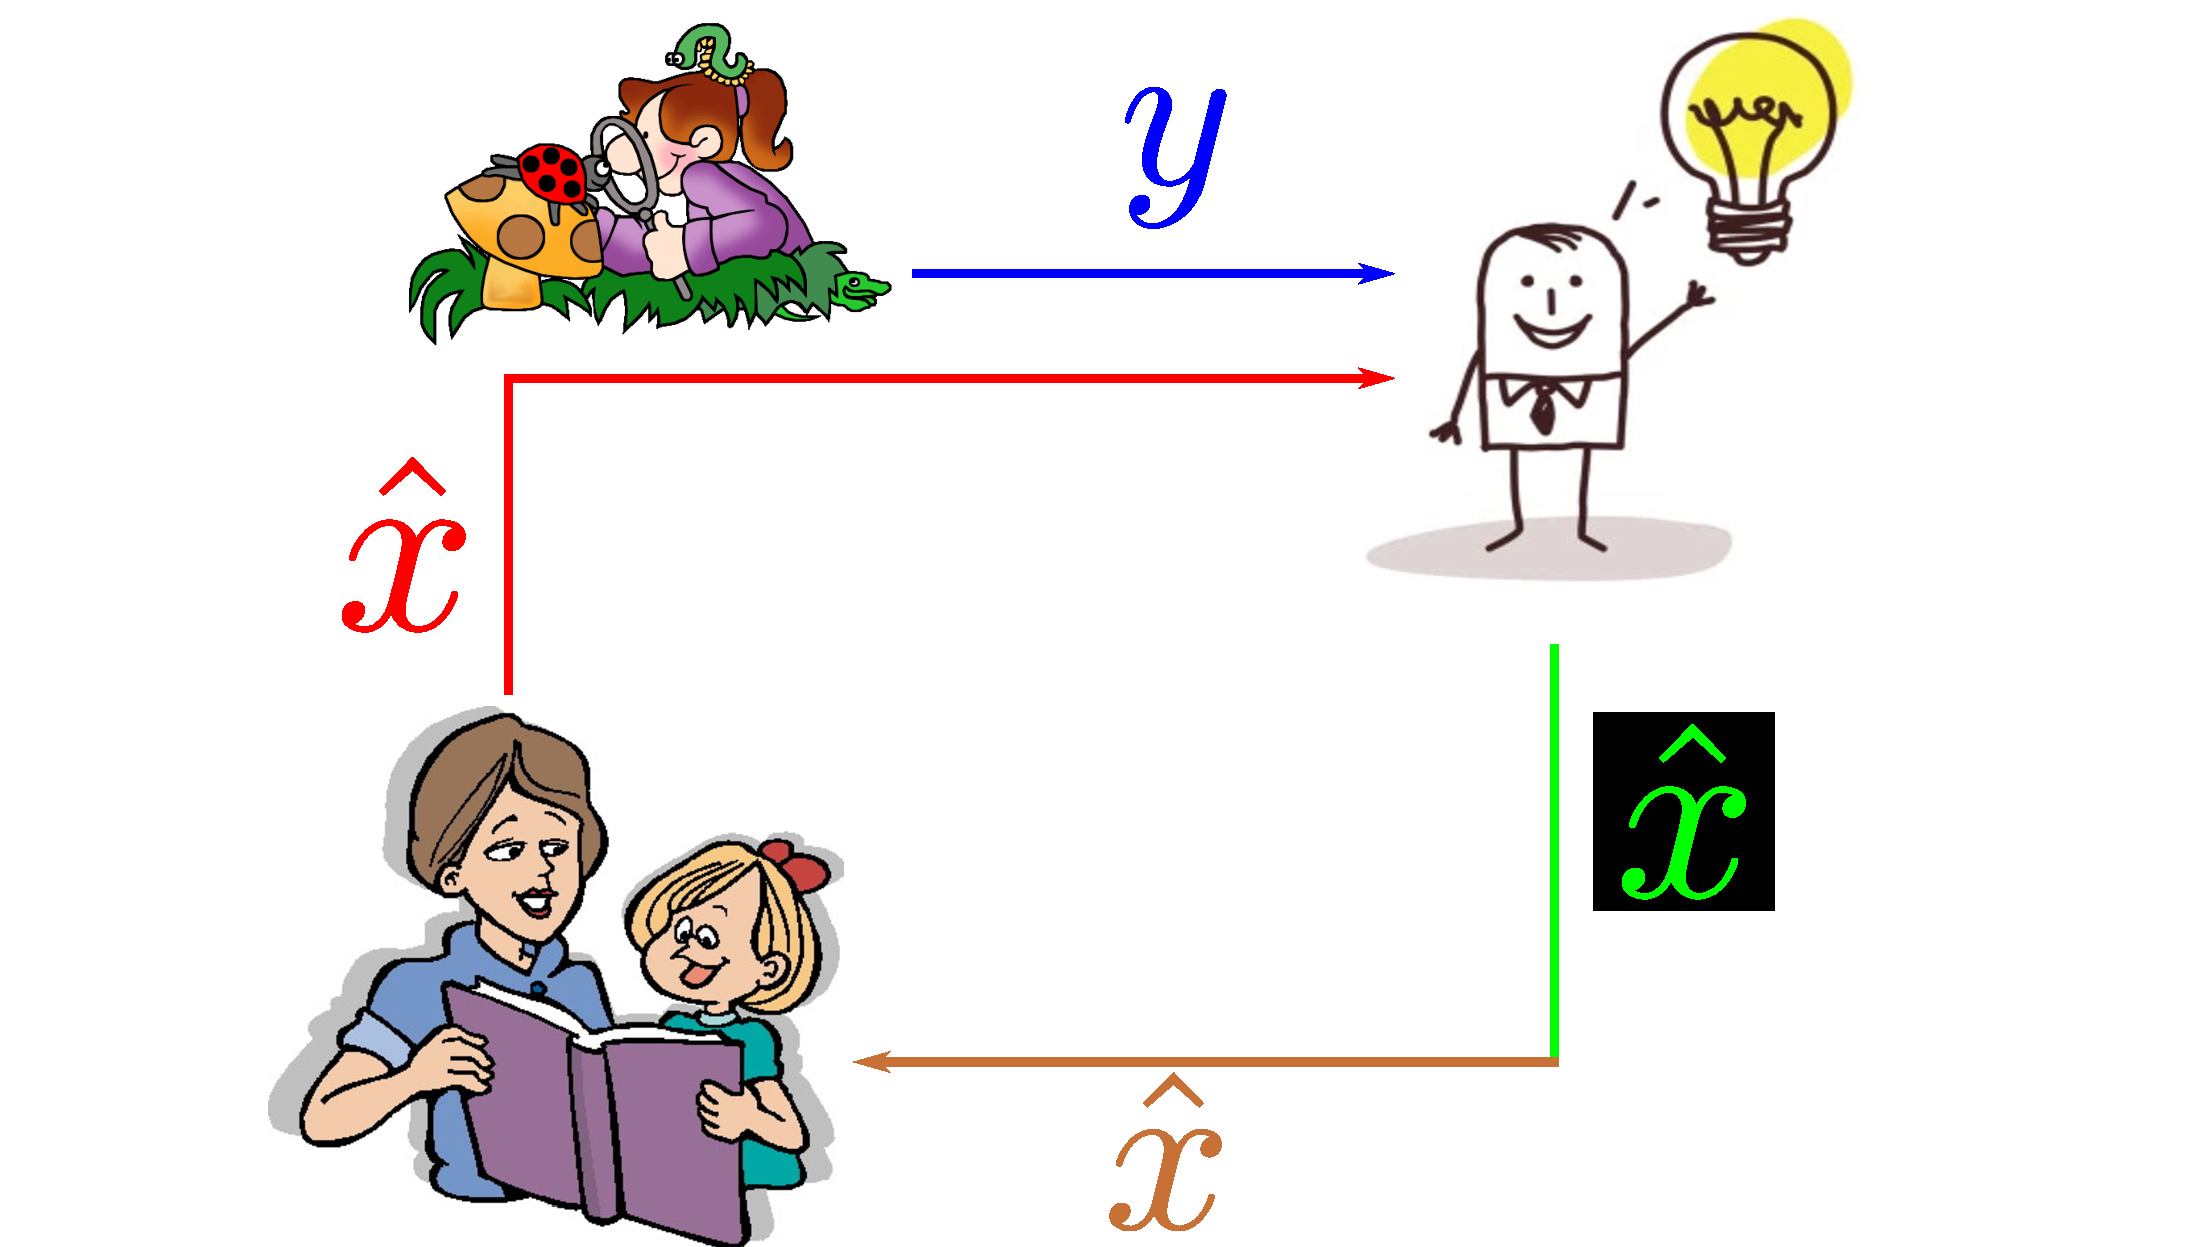
\includegraphics[width=0.95\textwidth]{figs/WFAR11_UCP_Update_Prediction_1_Notation-4.pdf}
\end{figure}
\end{frame}

%=================
\subsection{Problem Statement}
%=================
\begin{frame}\pw\Large
\frametitle{Overview}
\framesubtitle{}
\begin{figure}
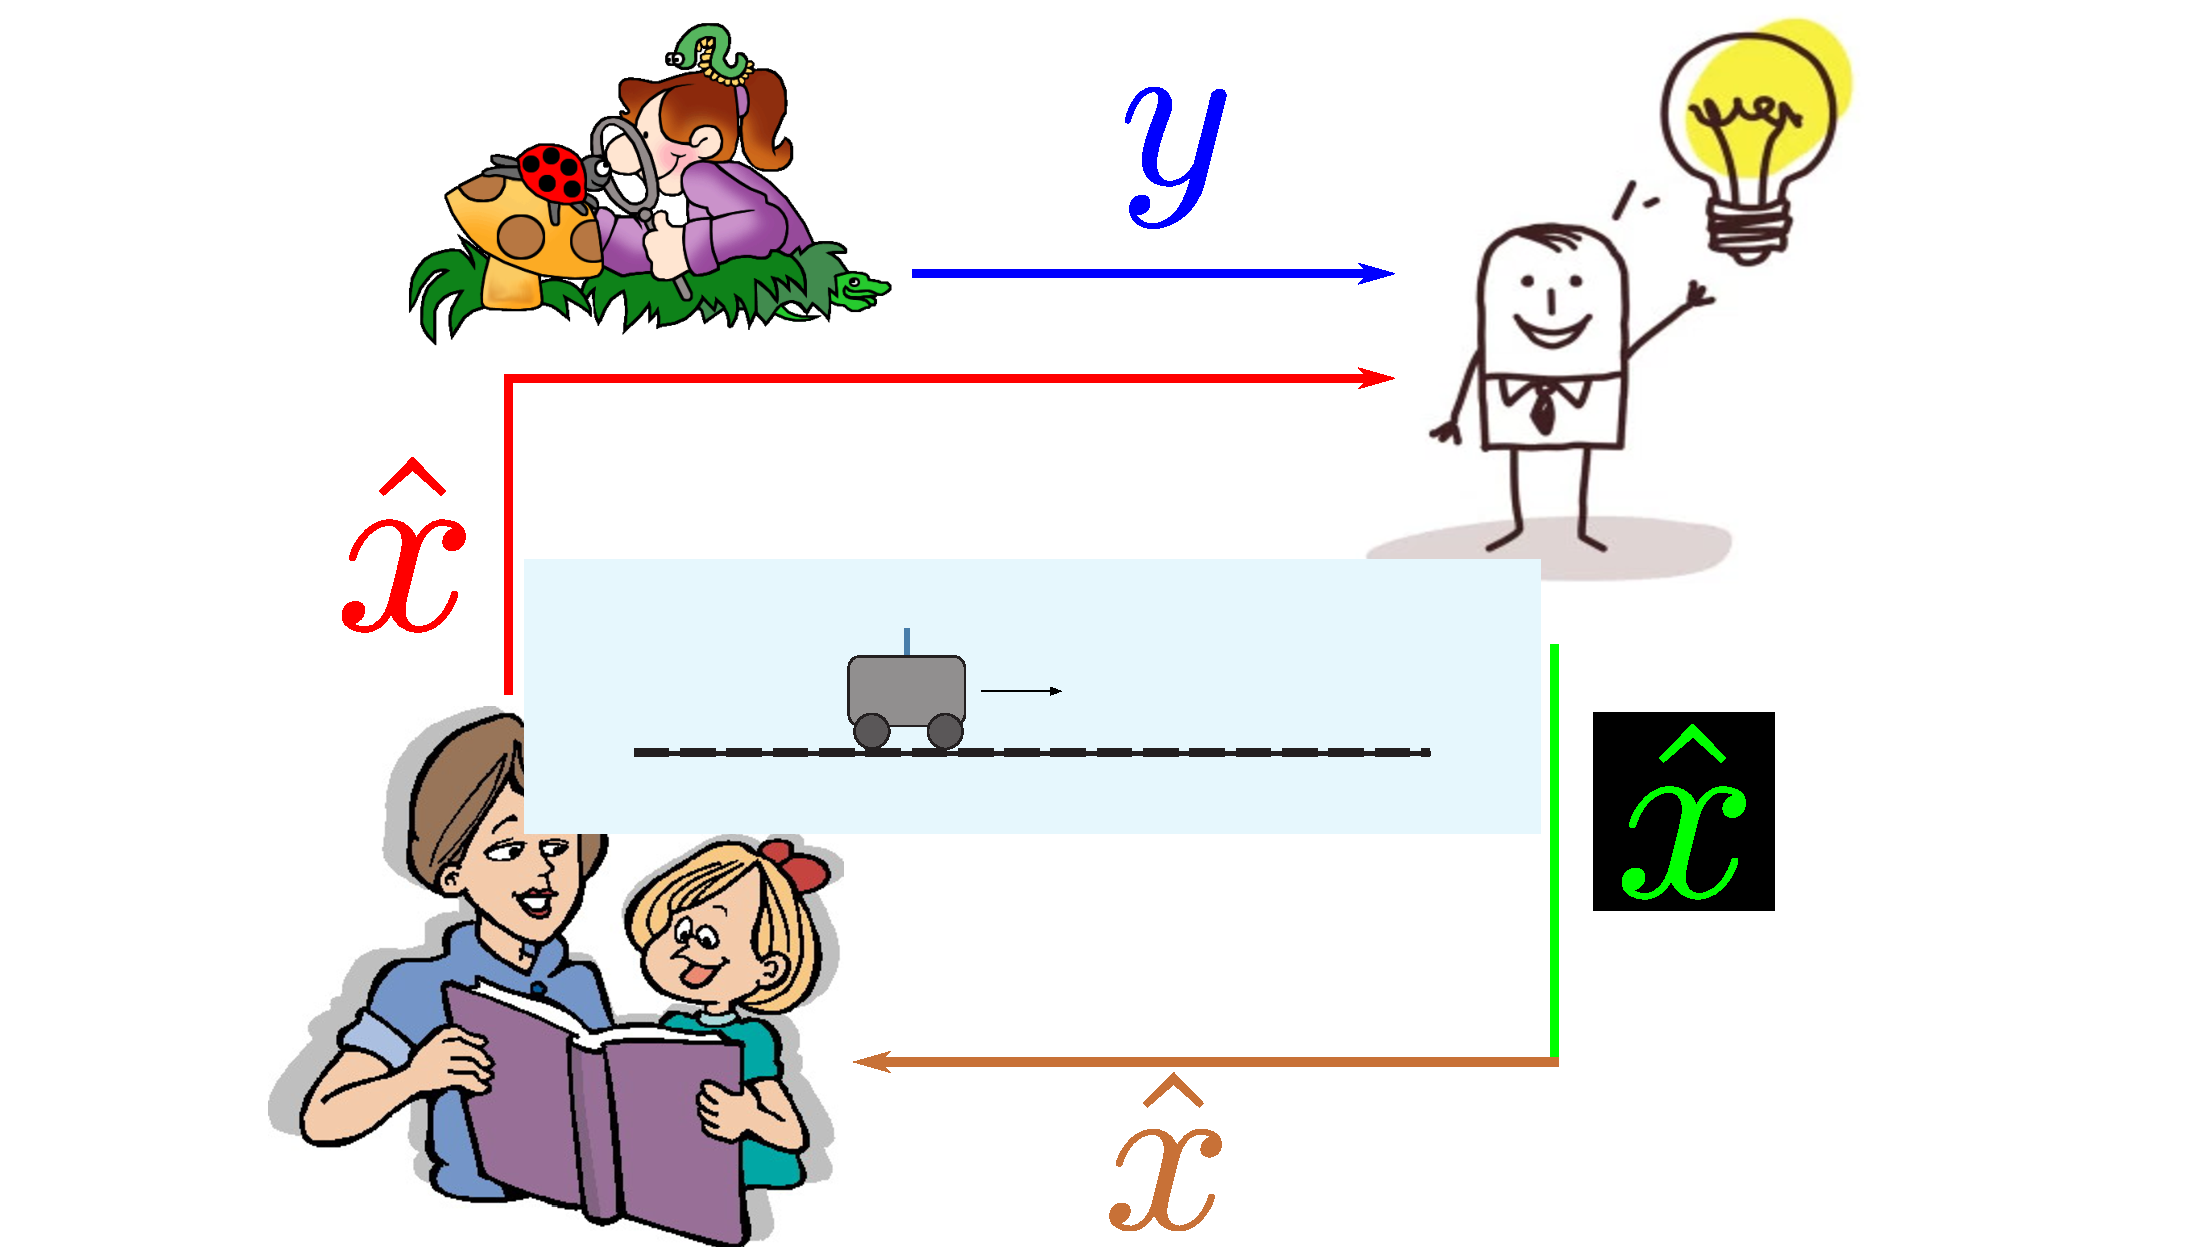
\includegraphics[width=0.95\textwidth]{figs/WFAR11_UCP_Update_Prediction_2_ProblemStatement-1.pdf}
\end{figure}
\end{frame}



\begin{frame}\pw\Large
\frametitle{Overview}
\framesubtitle{}
\begin{figure}
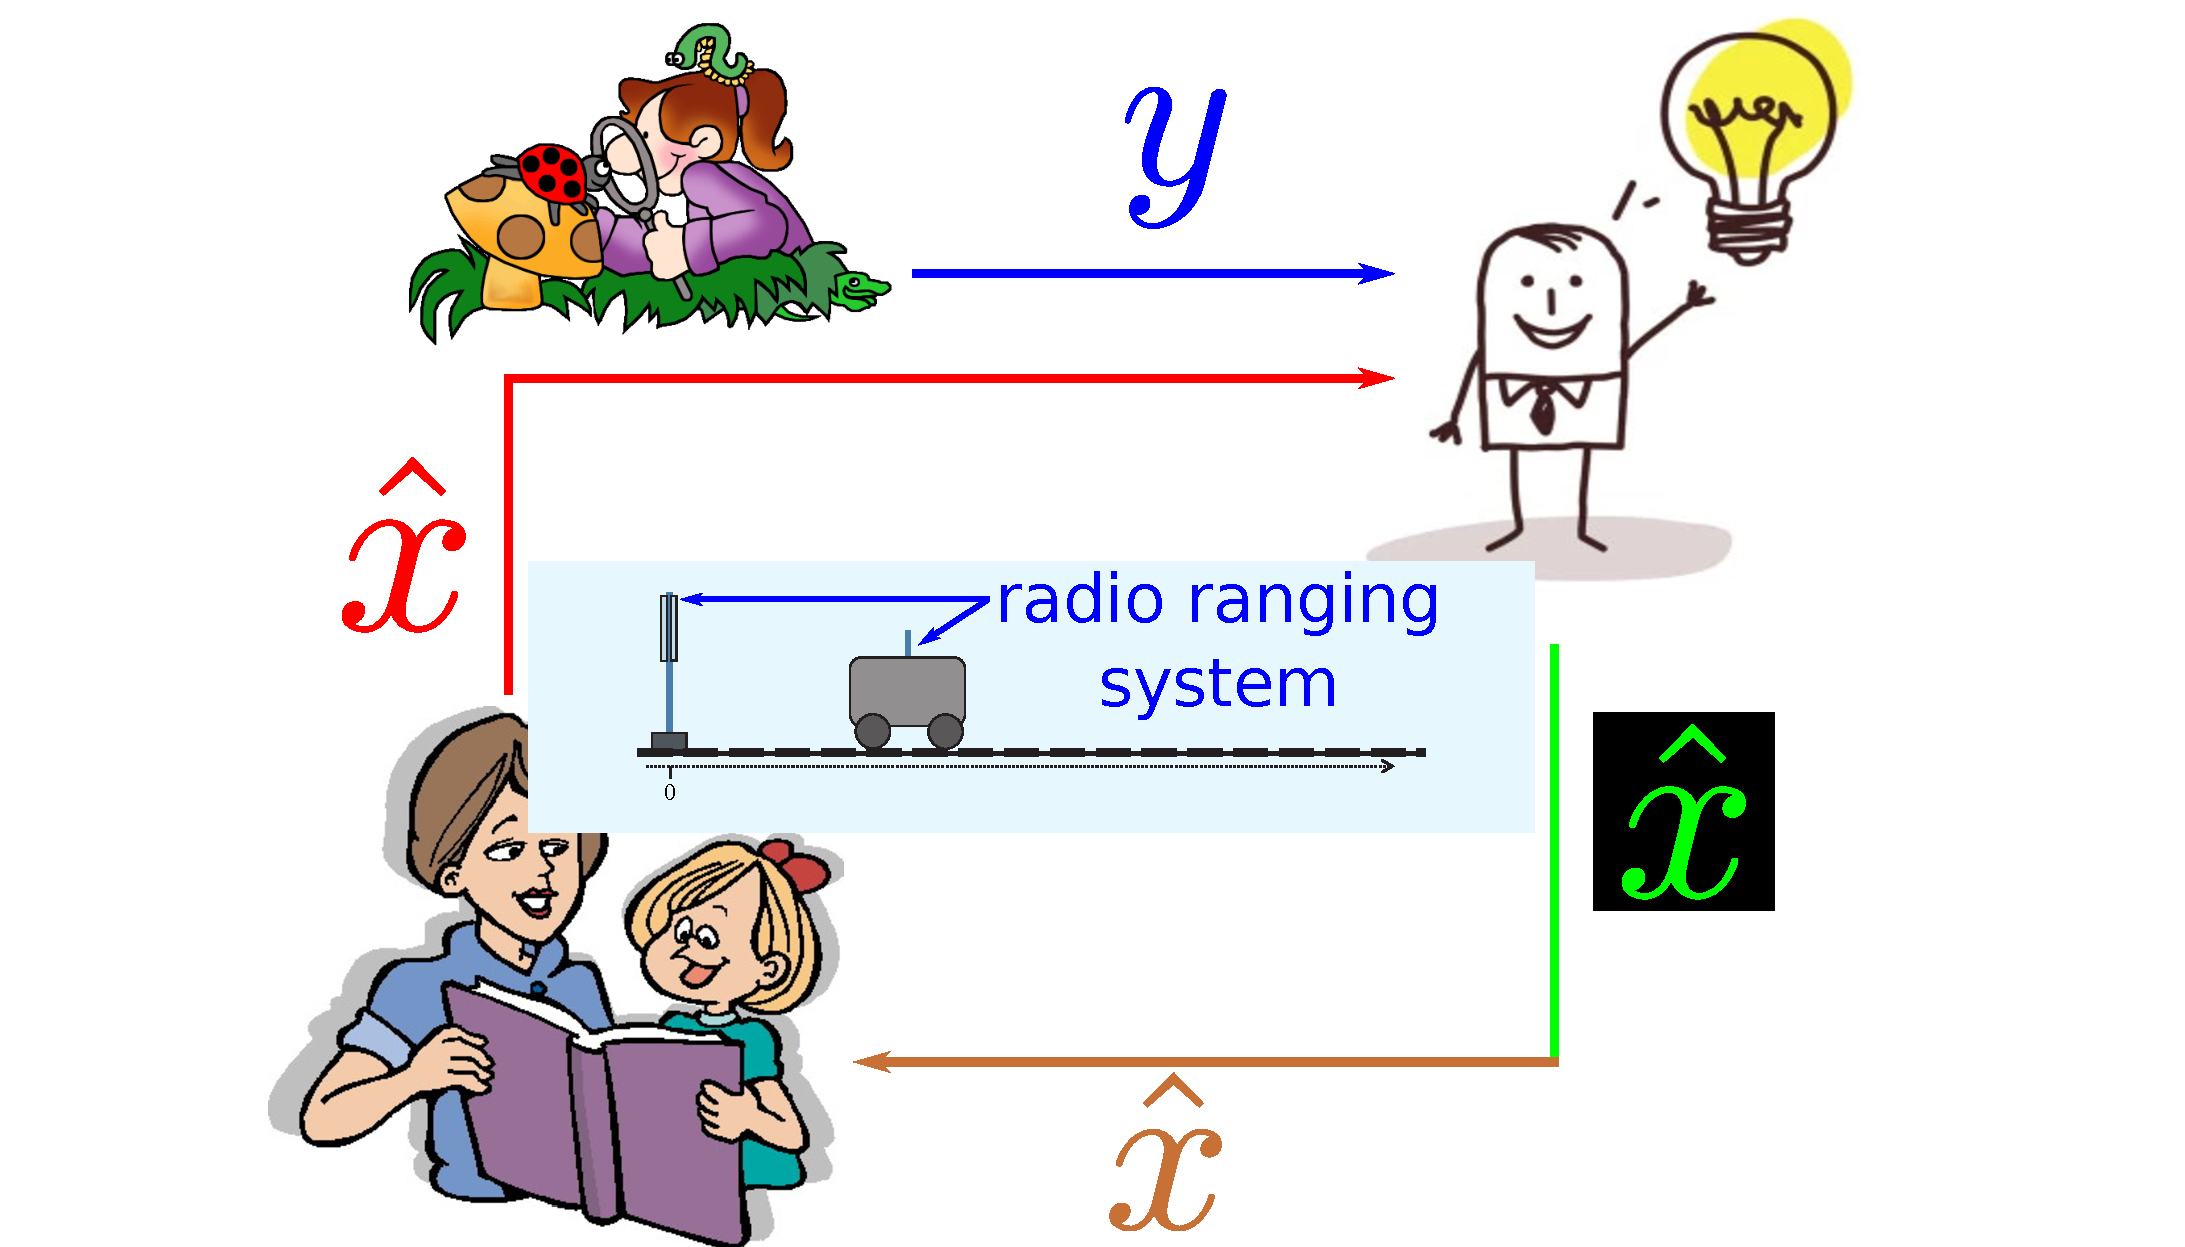
\includegraphics[width=0.95\textwidth]{figs/WFAR11_UCP_Update_Prediction_2_ProblemStatement-2.pdf}
\end{figure}
\end{frame}


%\begin{frame}\pw\Large
%\frametitle{Overview}
%\framesubtitle{}
%Combine {\color{red}expert opinion} and  {\color{red}observations} to come up with better {\color{green}understanding}
%\end{frame}



%###############
\section{Graphical Solution}
%###############
%=================
\subsection{Start}
%=================
\begin{frame}\pw\Large
\frametitle{Old Understanding}
\framesubtitle{}
\begin{figure}
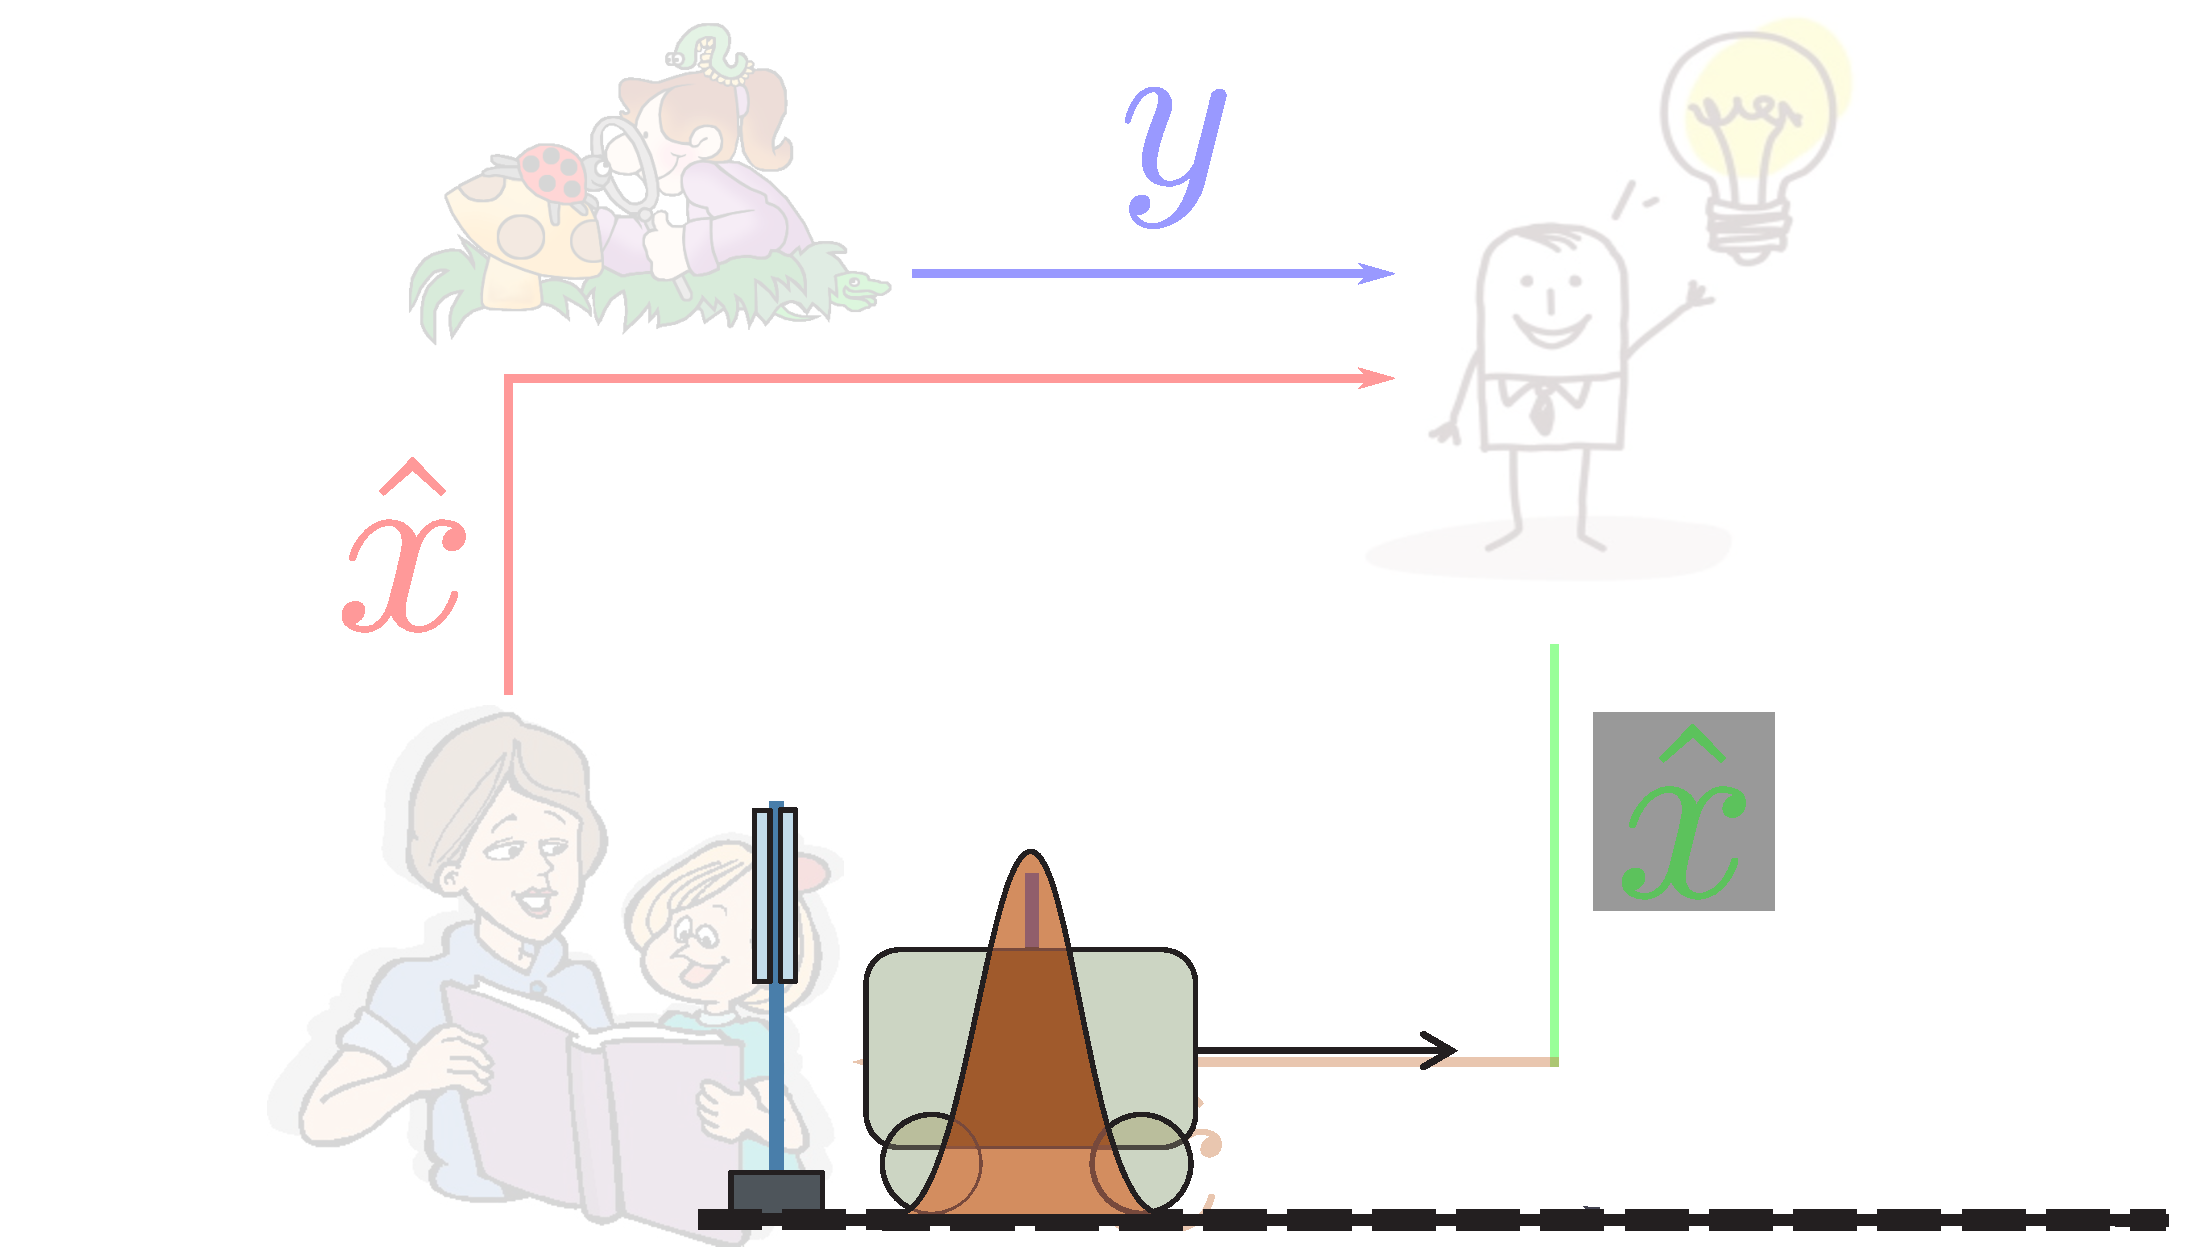
\includegraphics[width=0.95\textwidth]{figs/WFAR11_UCP_Update_Prediction_Process-0.pdf}
\end{figure}
\end{frame}



%=================
\subsection{Step 1}
%=================
\begin{frame}\pw\Large
\frametitle{Expectations}
\framesubtitle{}
\begin{figure}
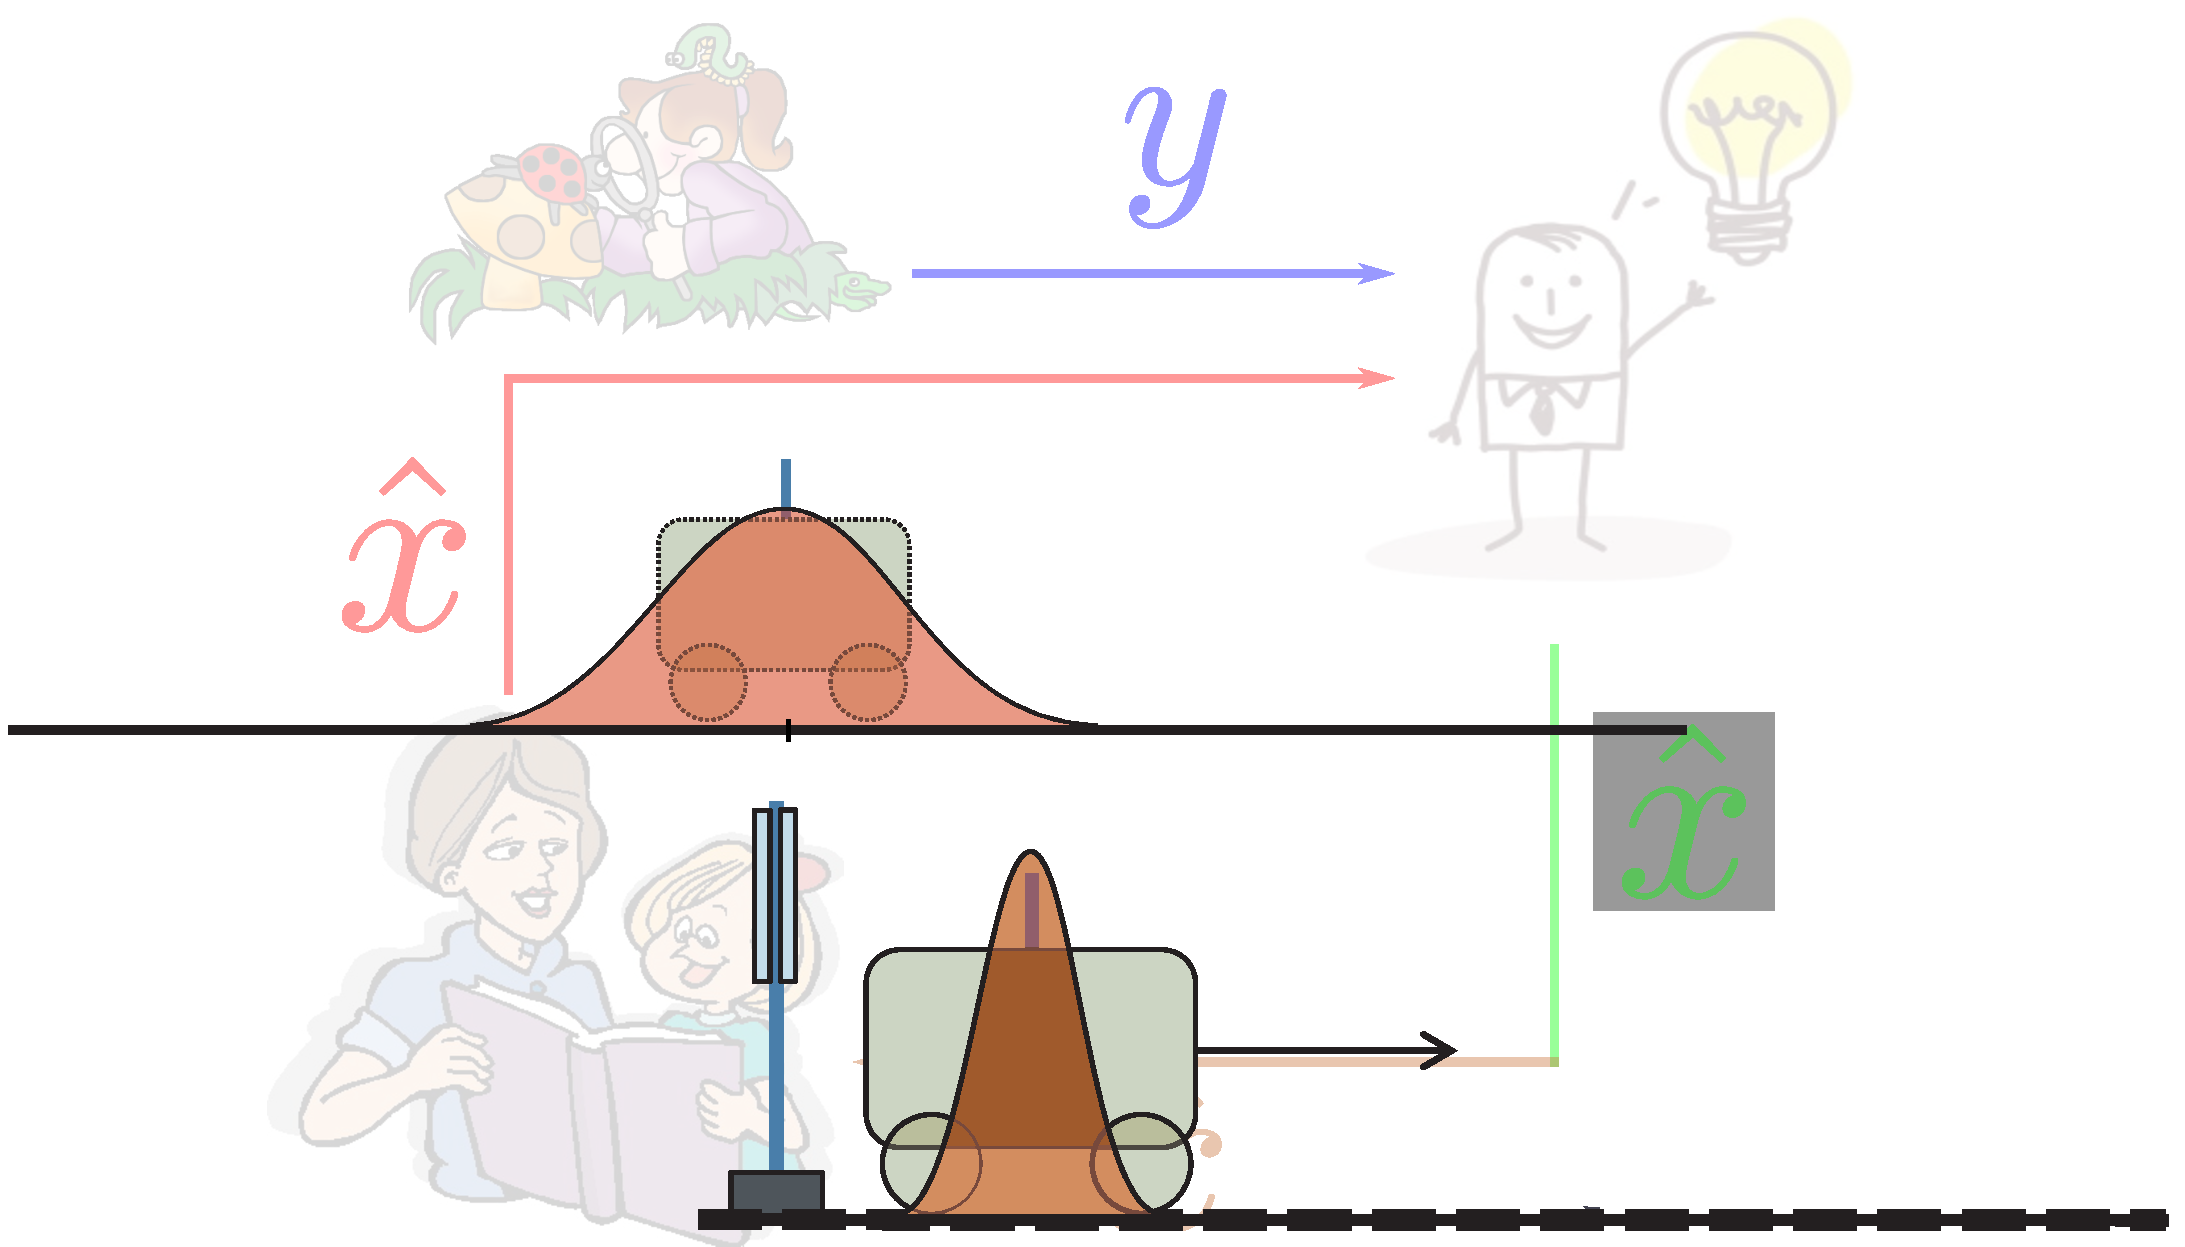
\includegraphics[width=0.95\textwidth]{figs/WFAR11_UCP_Update_Prediction_Process-1.pdf}
\end{figure}
\end{frame}


%=================
\subsection{Step 2}
%=================
\begin{frame}\pw\Large
\frametitle{Observations}
\framesubtitle{}
\begin{figure}
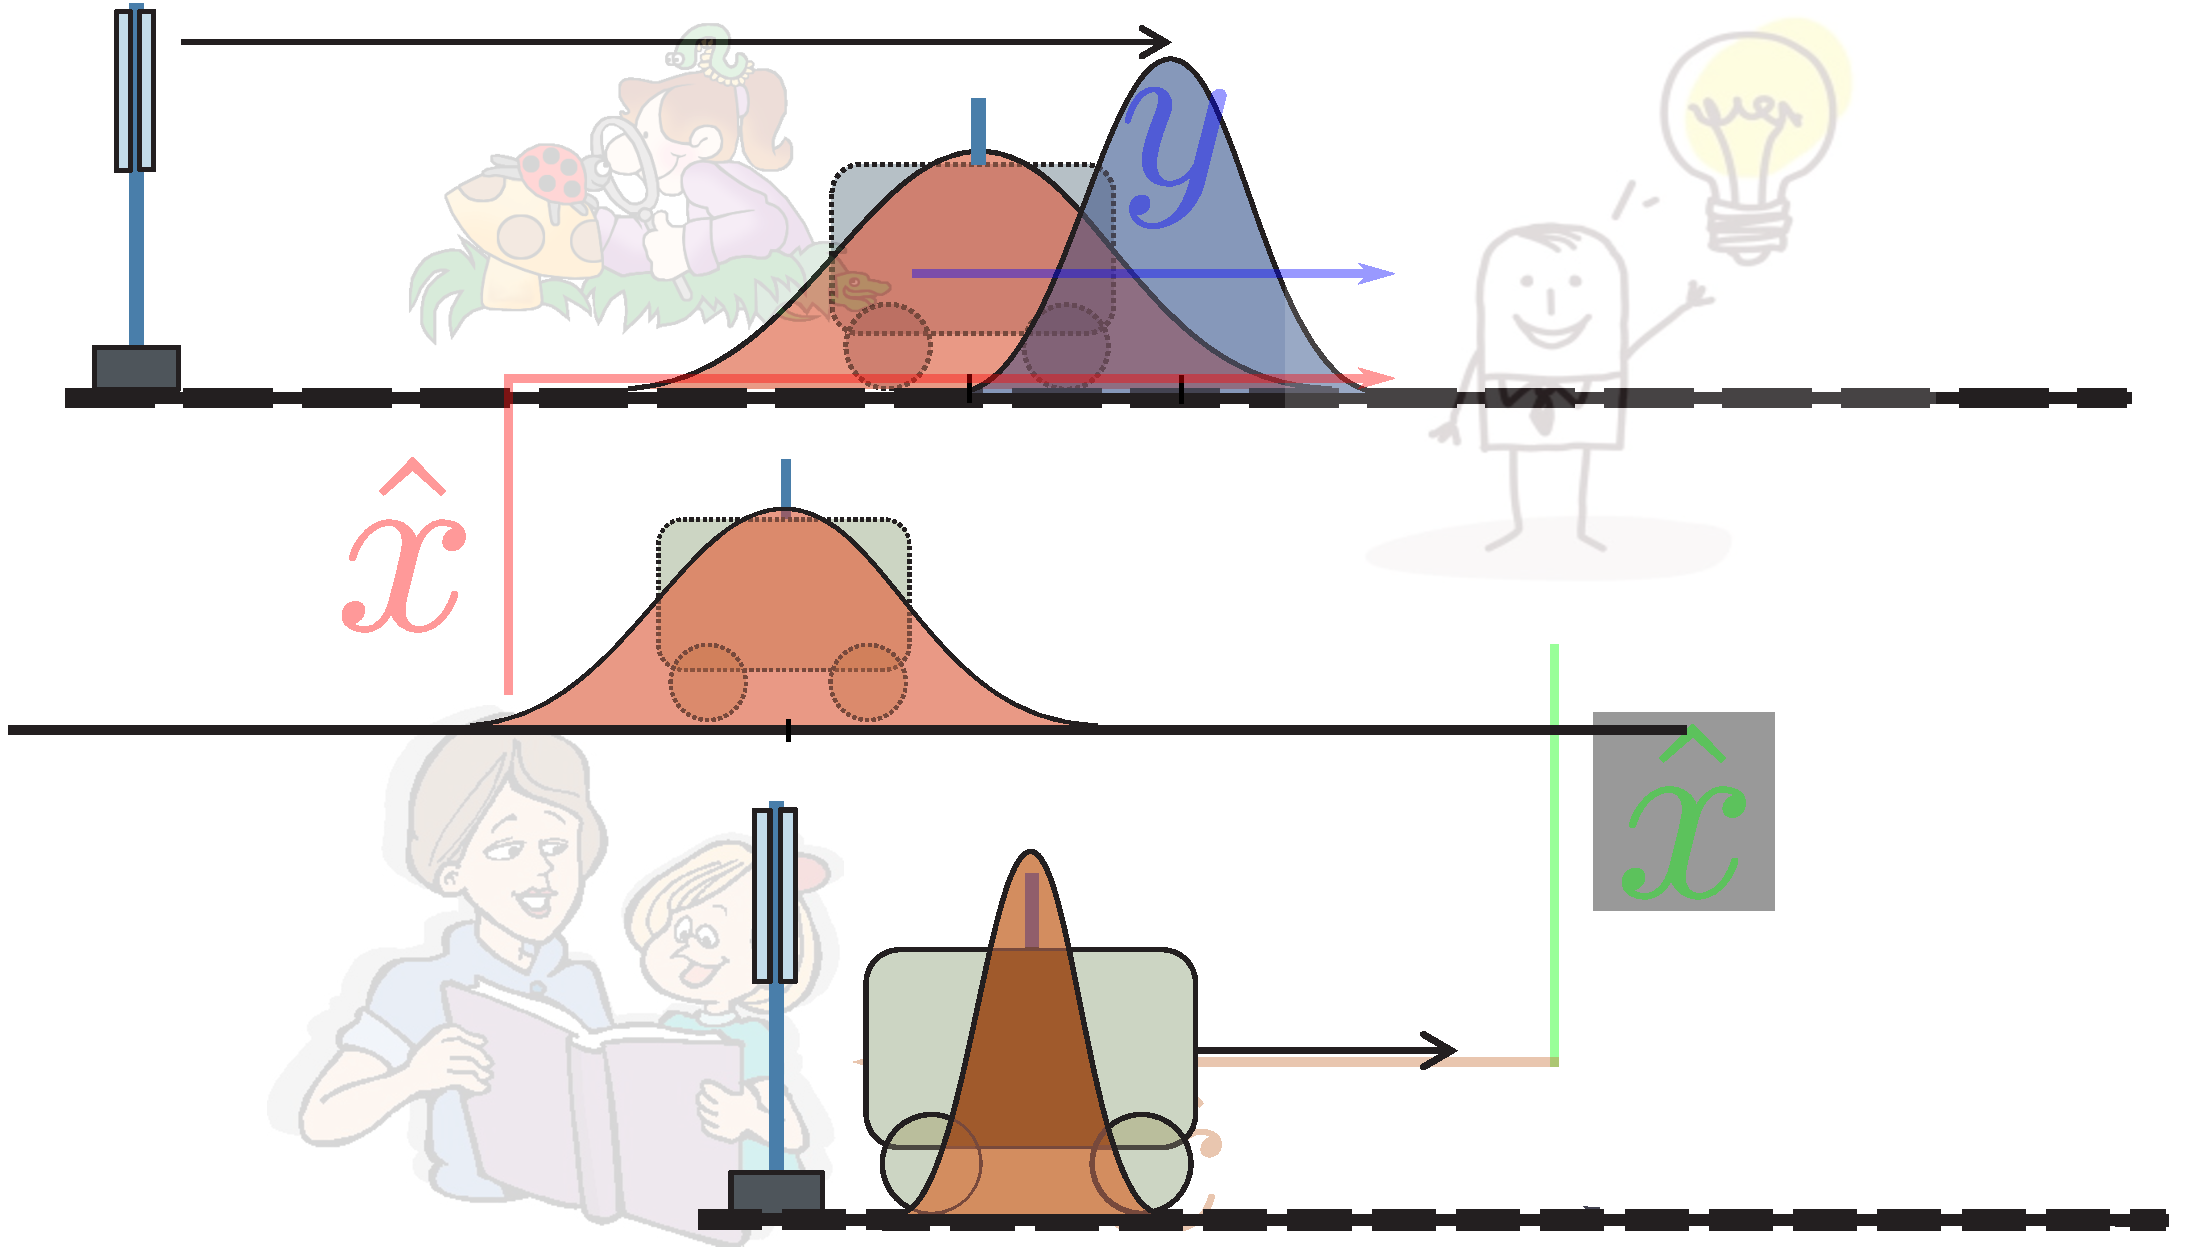
\includegraphics[width=0.95\textwidth]{figs/WFAR11_UCP_Update_Prediction_Process-2.pdf}
\end{figure}
\end{frame}


%=================
\subsection{Step 3}
%=================
\begin{frame}\pw\Large
\frametitle{New Understanding}
\framesubtitle{}
\begin{figure}
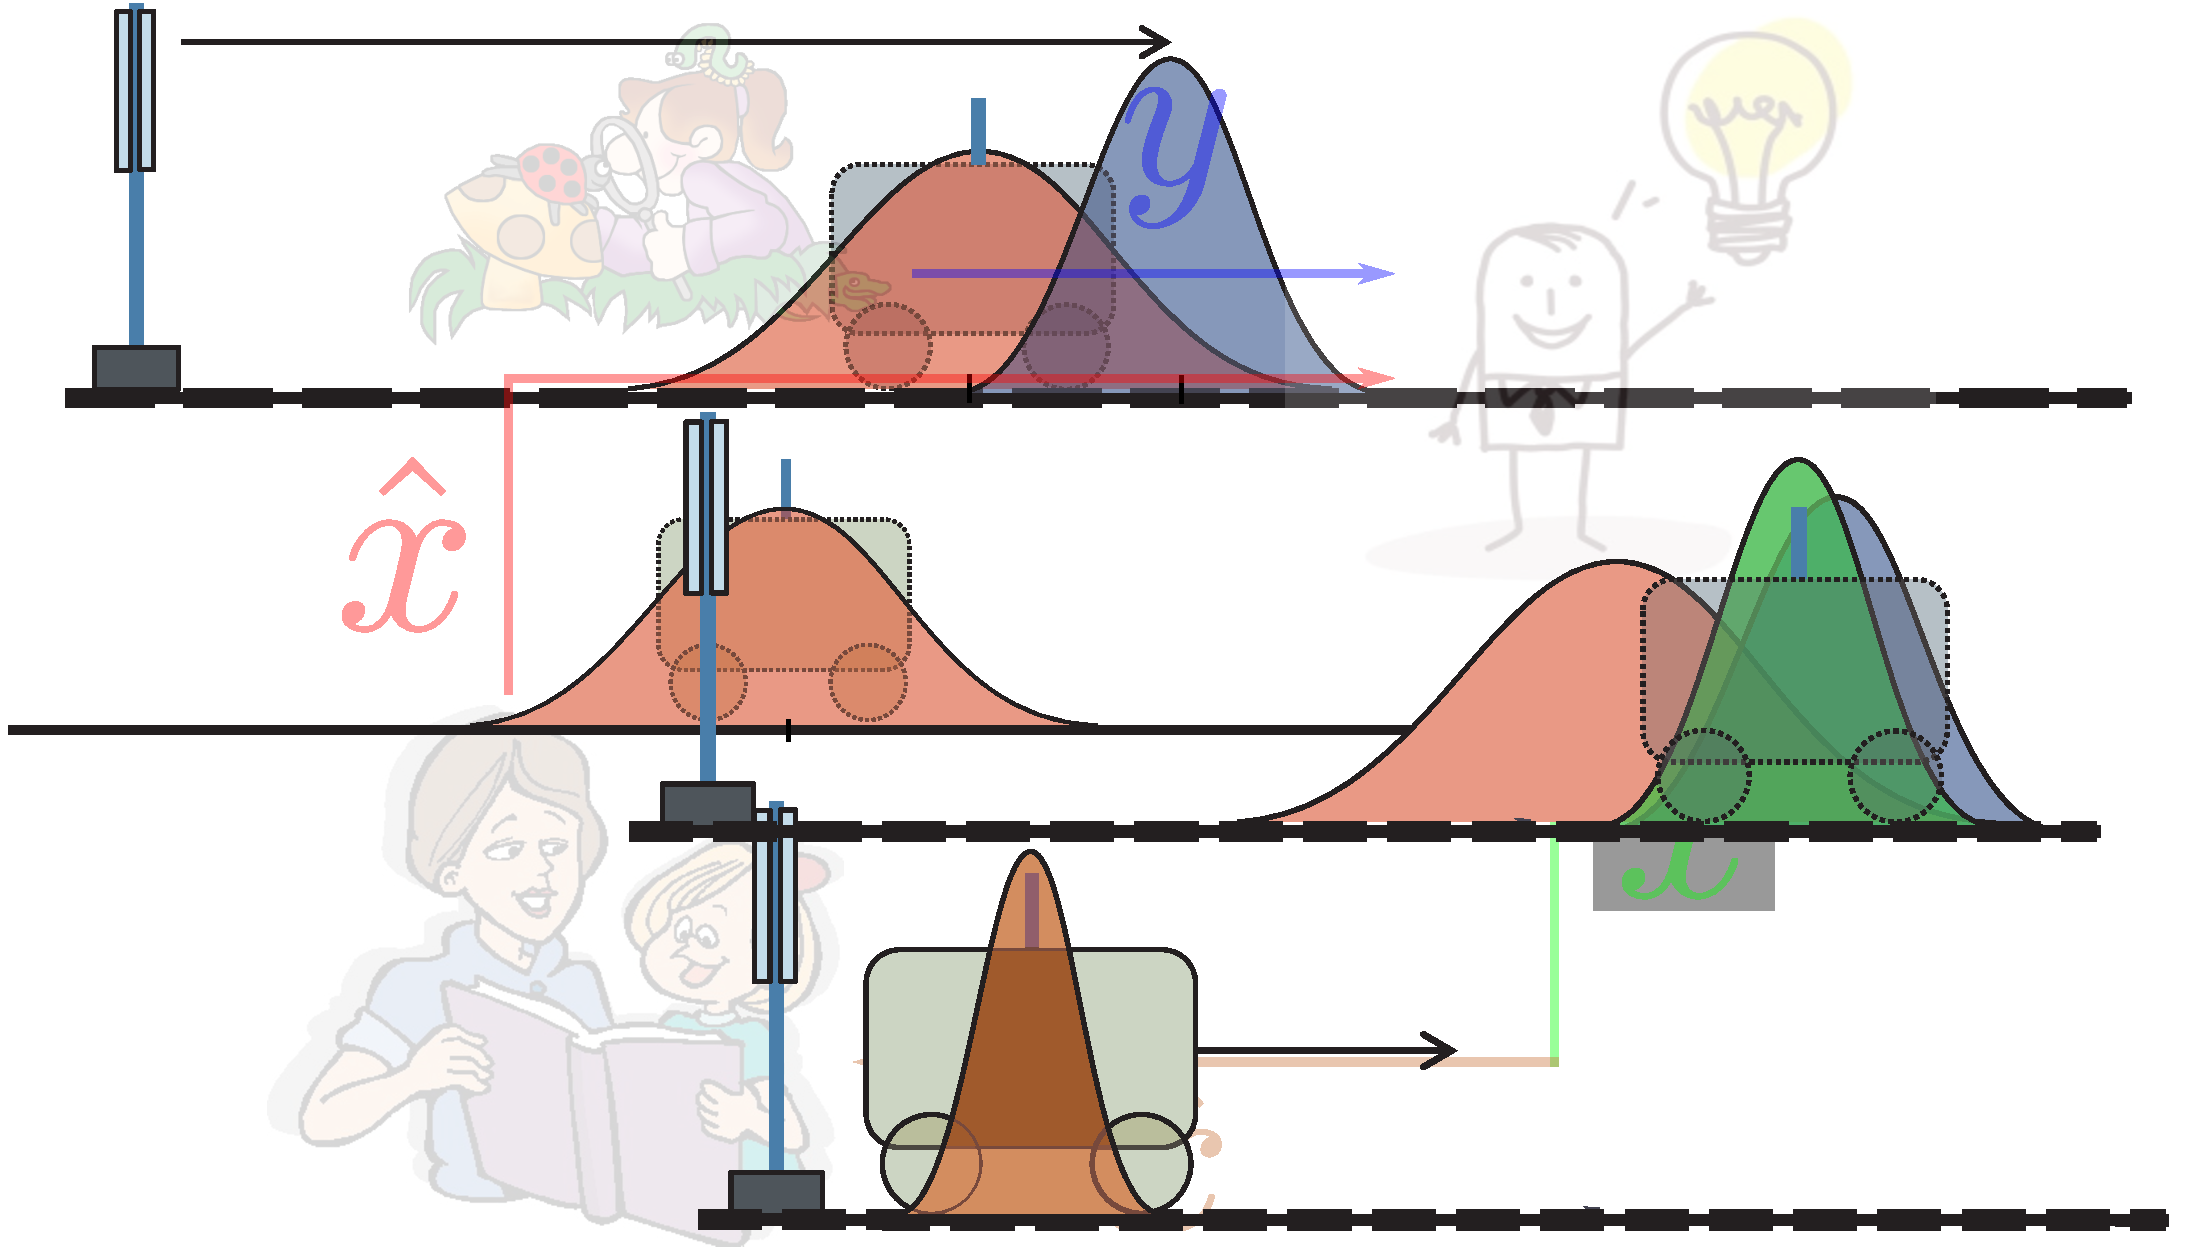
\includegraphics[width=0.95\textwidth]{figs/WFAR11_UCP_Update_Prediction_Process-3.pdf}
\end{figure}
\end{frame}


\begin{frame}\pw\Large
\frametitle{New Understanding}
\framesubtitle{}
\begin{figure}
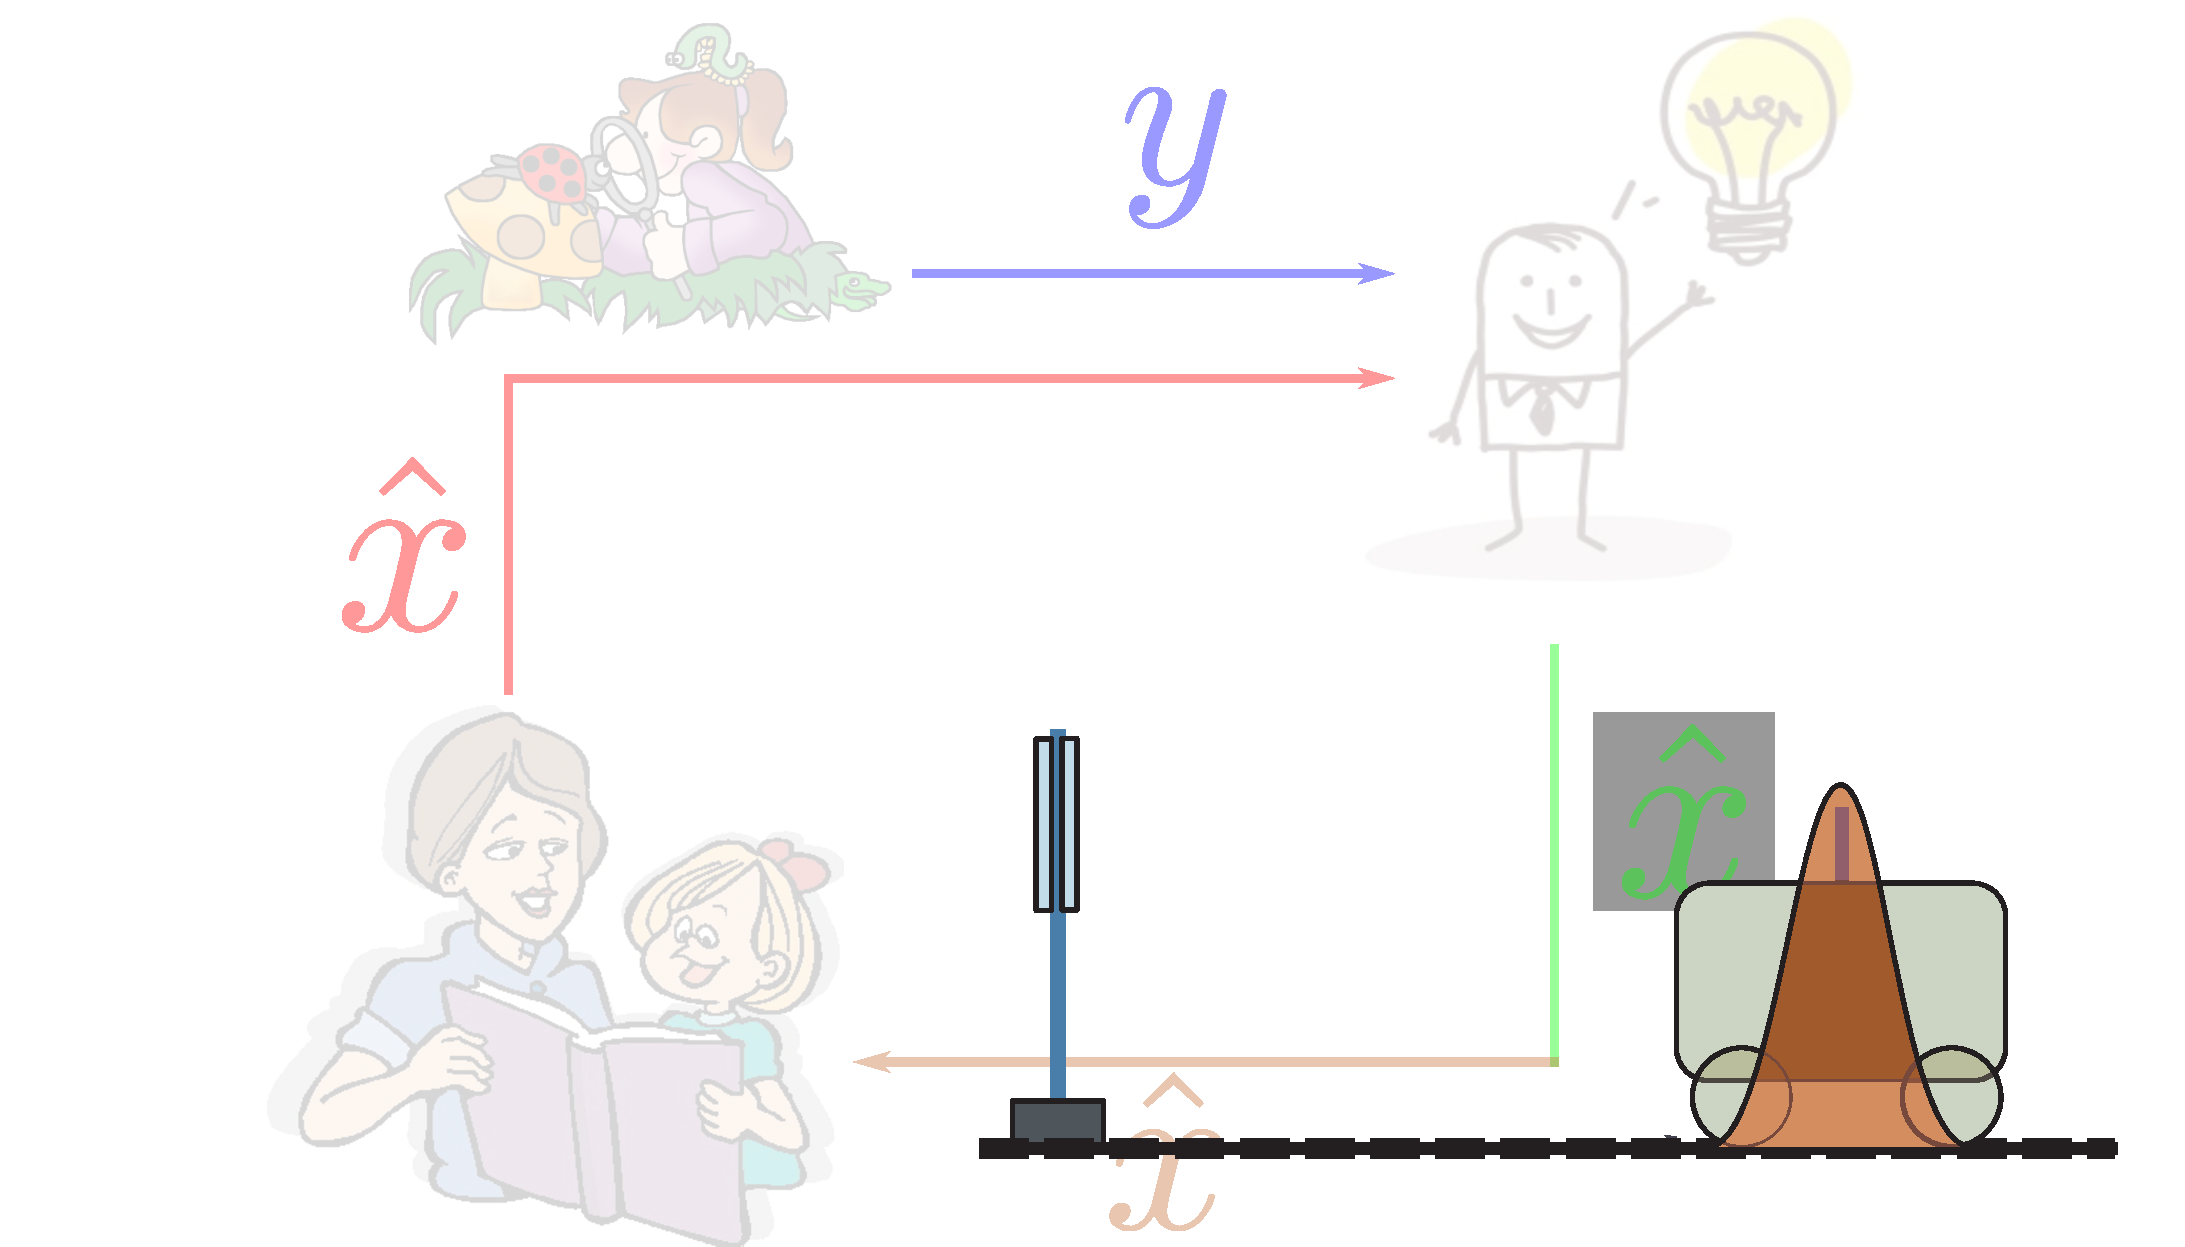
\includegraphics[width=0.95\textwidth]{figs/WFAR11_UCP_Update_Prediction_Process-4.pdf}
\end{figure}
\end{frame}

%###############
\section{Mathematical Solution}
%###############
%=================
\subsection{Scalar Case}
%=================
\begin{frame}\pw\Large
\frametitle{Derivation of Scalar Case}
\framesubtitle{}
Let $p_1$ and $p_2$ be two Gaussian pdfs:
\begin{equation*}
\begin{array}{llll}
p_1(x; \muone, \sone)&=\frac{1}{\sqrt{2 \pi \varone}} e^{-\frac{(x-\muone)^2}{2 \varone}}\\
p_2(x; \mutwo, \stwo)&=\frac{1}{\sqrt{2 \pi \vartwo}} e^{-\frac{(x-\mutwo)^2}{2 \vartwo}}\\\\
\end{array}
\end{equation*}
Their product is:
\begin{equation*}
\begin{array}{llll}
p_1p_2 &=     \frac{1}{\sqrt{2 \pi \varone}} e^{-\frac{(x-\muone)^2}{2 \varone}}    \frac{1}{\sqrt{2 \pi \vartwo}} e^{-\frac{(x-\mutwo)^2}{2 \vartwo}}\\\\
\end{array}
\end{equation*}
where ${\color{Orange}K}=\frac{C\varone}{C^2\varone + \vartwo}$
\end{frame}



%\begin{frame}\pw\Large
%\frametitle{Derivation of Scalar Case}
%\framesubtitle{}
%Combining exponents
%\begin{equation*}
%\begin{array}{llll}
%&=\frac{1}{\sqrt{2 \pi \varone \vartwo 2 \pi }}         e^{ -\frac{(x-\muone)^2}{2 \varone} - \frac{(x-\mutwo)^2}{2 \vartwo} } \\\\
%\end{array}
%\end{equation*}
%Taking LCM
%\begin{equation*}
%\begin{array}{llll}
%&=    \frac{1}{\sqrt{2 \pi \varone \vartwo 2 \pi }}         e^{ \frac{ - \vartwo (x-\muone)^2 - \varone (x-\mutwo)^2 } { 2 \varone \vartwo } }\\
%\end{array}
%\end{equation*}
%\end{frame}



\begin{frame}\pw\Large
\frametitle{Derivation of Scalar Case}
\framesubtitle{}
$p_1p_2$ will be a Gaussian function with mean
\begin{equation*}
\begin{array}{rlllllll}
\mufused &= \frac { \muone \vartwo + \mutwo \varone }{\varone + \vartwo}\\
 &= \frac { \muone \vartwo + \mutwo C\varone }{C^2\varone + \vartwo}\\
&=\muone + \frac{\varone(C\mutwo-C^2\muone)}{C^2\varone + \vartwo}\\
&=\muone + \frac{C\varone(\mutwo-C\muone)}{C^2\varone + \vartwo} =\muone  + {\color{Orange}K}(\mutwo-C\muone)
\end{array}
\end{equation*}
\end{frame}





\begin{frame}\pw\Large
\frametitle{Derivation of Scalar Case}
\framesubtitle{}
And variance
\begin{equation*}
\begin{array}{rlllllll}
\varfused
&= \frac{\varone \vartwo}{\varone + \vartwo}\\
&= \frac{\varone \vartwo}{C^2\varone + \vartwo}\\
&=\varone - \frac{C^2\color{red}\sigma^4_1}{C^2\varone + \vartwo}\\
&=\varone-\frac{C\varone}{C^2\varone + \vartwo}C\varone\\
&=(1-{\color{Orange}K}C)\varone\\\\
\end{array}
\end{equation*}
where ${\color{Orange}K}$ is the same as defined in the previous slide
\end{frame}



%=================
\subsection{Comparison With Vector Case}
%=================
\begin{frame}\pw\Large
\frametitle{One-to-one Correspondence}
\framesubtitle{}
\begin{figure}[h]
\centering
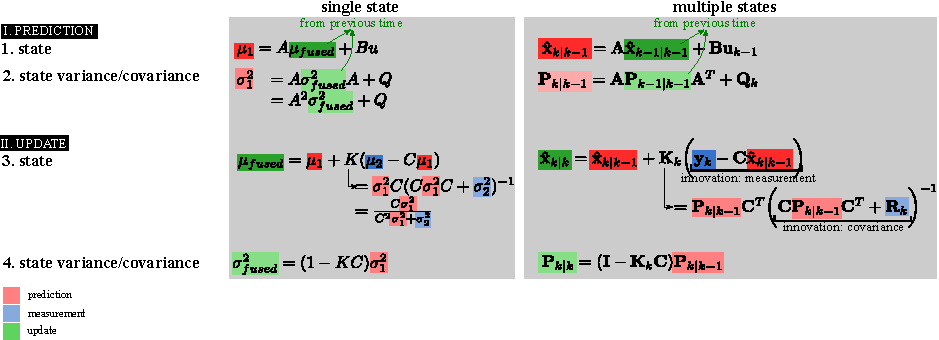
\includegraphics[width=1.07\textwidth]{figs/TRK_KalmanFilter_equations-2D.pdf}
\end{figure}
\end{frame}




%###############
\section{Programmatical Solution}
%###############

\begin{frame}[fragile, allowframebreaks]\pw\Large
\frametitle{Matlab Code}
\framesubtitle{}

\scriptsize
The code below implements 2 time steps for the train:
\tinyvvv \begin{lstlisting}[language=Matlab]
clear;clc;clf;

%initialization
x           =   -5:0.1:25;  %x axis
A           =   2;          %state transition matrix
B           =   5;          %control input matrix
C           =   1;          %transformation matrix
u           =   1;          %control input
Q           =   1.2;        %process noise variance, adds uncertainty to prediction
mu_2        =   [7 14];     %the output of the radio ranging system at next two times
var_2       =   1;          %the variance of the radio ranging system given by manufacturer

mu_f        =   0;          %the estimated location of the train at current time, k=0
var_f       =   1;          %the estimated variance of our estimate at current time, k=0

pdf_0       =   (1/sqrt(2*pi*var_f))*exp(-(0.5/var_f)*(x-mu_f).^2);


%=====================================
%run Kalman Filter
%=====================================
for k=1:2
    %predict
    mu_1        =   A*mu_f      +   B*u;
    var_1       =   A^2*var_f   +   Q;
    %update
    K           =   (C*var_1)/(C^2*var_1 + var_2);
    mu_f        =   mu_1 + K*(mu_2(k)-C*mu_1);
    var_f       =   (1-K*C)*var_1;
    
    pred        =   (1/sqrt(2*pi*var_1))*exp(-(0.5/var_1)*(x-mu_1).^2);
    meas        =   (1/sqrt(2*pi*var_2))*exp(-(0.5/var_2)*(x-mu_2(k)).^2);
    fused       =   (1/sqrt(2*pi*var_f))*exp(-(0.5/var_f)*(x-mu_f).^2);
    
                    axis([-5 25 0 0.5]); 
                    grid on;
                    hold on;


                    plot(x,pred, 'r--x');
                    plot(x,meas, 'b--o');
                    plot(x,fused,'g--.')
                    plot(x,pdf_0,'g--.');                    
end
legend('predicted', 'measured', 'fused')
xlabel('railway track (meters), direction along which train is traveling ->')
ylabel('belief in fused/predicted/measured position of train')
title('Data fusion using the Kalman Filter')
\end{lstlisting}
\end{frame}








\begin{frame}\pw\Large
\frametitle{Results}
\framesubtitle{}
The code on the previous slide produces this output:
\begin{figure}[h]
\centering
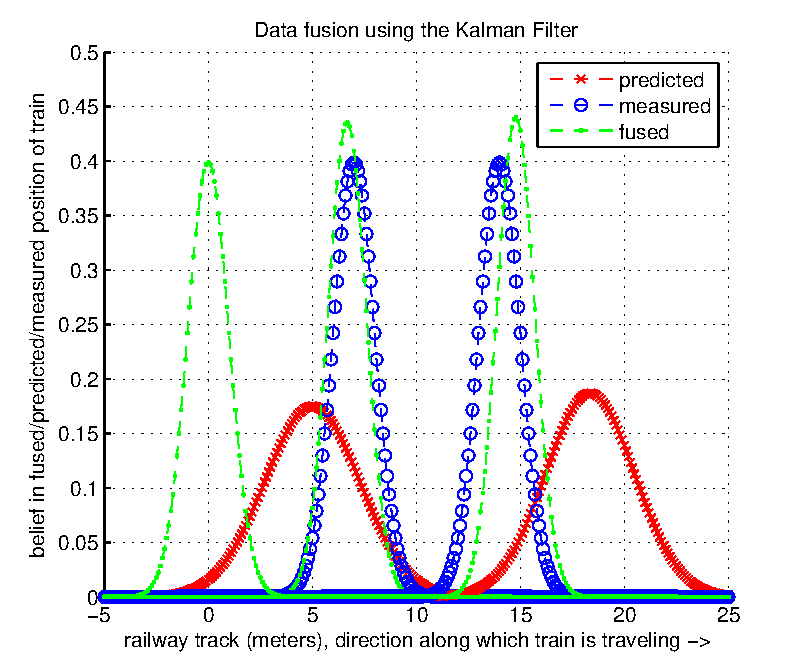
\includegraphics[width=0.47\textwidth]{figs/CONTROLS_Kalman_train_example.pdf}
\caption{\tiny In this example, a train is moving along the x-axis.  The problem begins at time $kT=0$ sec when our initial estimate of the train is that it is standing at $x=0$ meters.  The prediction and measurements for the next two time instants, $kT=1$ sec and $kT=2$ sec are shown.  We assume for simplicity but without loss of generality, that $T=1$~sec, and therefore we use $k$ (in sec) to depict time.  It may be mentioned that the version of the Kalman filter for continuous time is called the Kalman-Bucy filter.}
\end{figure}
\end{frame}


%###############
\appendix
%###############
\begin{frame}\Large
\frametitle{}
\framesubtitle{}
Questions
\end{frame}

%##################################
\end{document}
%##################################